\documentclass[sigconf]{acmart}
\AtBeginDocument{%
  \providecommand\BibTeX{{%
    \normalfont B\kern-0.5em{\scshape i\kern-0.25em b}\kern-0.8em\TeX}}}

\copyrightyear{2022}
\acmYear{2022}
\setcopyright{acmlicensed}
\acmConference[Web3D '22]{The 27th International Conference on 3D Web Technology}{November 2--4, 2022}{Evry-Courcouronnes, France}
\acmBooktitle{The 27th International Conference on 3D Web Technology (Web3D '22), November 2--4, 2022, Evry-Courcouronnes, France}
\acmPrice{15.00}
\acmDOI{10.1145/3564533.3564566}
\acmISBN{978-1-4503-9914-2/22/11}

\acmSubmissionID{13}
\citestyle{acmauthoryear}

\usepackage{subcaption}
\usepackage{csquotes}


\usepackage{calc}
\usepackage{tikz}
\usetikzlibrary{calc,positioning,spy,shapes}

\tikzset{thick/.style = {line width = 1.0pt}}

\newlength{\pfull}  \setlength{\pfull}  {2mm}
\newlength{\phalf}  \setlength{\phalf}  {0.5\pfull}

\newlength{\lwffp}   \setlength{\lwffp}   {0.5000\dimexpr(\linewidth-1.0\pfull)}
\newlength{\lwfffp}  \setlength{\lwfffp}  {0.3333\dimexpr(\linewidth-2.0\pfull)}
\newlength{\lwffffp} \setlength{\lwffffp} {0.2500\dimexpr(\linewidth-3.0\pfull)}
\newlength{\lwfffffp}\setlength{\lwfffffp}{0.2000\dimexpr(\linewidth-4.0\pfull)}

\newlength{\twffp}   \setlength{\twffp}   {0.5000\dimexpr(\textwidth-1.0\pfull)}
\newlength{\twfffp}  \setlength{\twfffp}  {0.3333\dimexpr(\textwidth-2.0\pfull)}
\newlength{\twffffp} \setlength{\twffffp} {0.2500\dimexpr(\textwidth-3.0\pfull)}
\newlength{\twfffffp}\setlength{\twfffffp}{0.2000\dimexpr(\textwidth-4.0\pfull)}

\tikzstyle{labelStyle} = [ shape = rectangle, font = \scriptsize, text depth = 0, fill = white, inner sep = 4pt ]
\tikzstyle{labelN}  = [ labelStyle, anchor = north ]
\tikzstyle{labelNW} = [ labelStyle, anchor = north west ]
\tikzstyle{labelNE} = [ labelStyle, anchor = north east ]
\tikzstyle{labelS}  = [ labelStyle, anchor = south ]
\tikzstyle{labelSW} = [ labelStyle, anchor = south west ]
\tikzstyle{labelSE} = [ labelStyle, anchor = south east ]

\tikzstyle{figRC} = [shape = rectangle, rounded corners = 2mm, clip] %
\tikzstyle{spyRC} = [shape = rectangle, rounded corners = 2mm, %
    white, connect spies, every spy on node/.append style = {thick}] %
\tikzstyle{figNS} = [inner sep = 0pt, outer sep = 0pt] %
 %

\usetikzlibrary{external}
\tikzset{external/system call={pdflatex \tikzexternalcheckshellescape -halt-on-error -interaction=batchmode -jobname "\image" "\texsource"}}
\tikzsetexternalprefix{figures/}
\tikzset{external/only named=true}
\tikzexternalize %

\usepackage{pgfplots}
\pgfplotsset{compat=1.18}

\makeatletter
\newcommand{\gettikzxy}[3]{%
  \tikz@scan@one@point\pgfutil@firstofone#1\relax
  \edef#2{\the\pgf@x}%
  \edef#3{\the\pgf@y}%
}
\makeatother

\definecolor{viridisA}{HTML}{91bfdb}
\definecolor{viridisB}{HTML}{e0f3f8}
\definecolor{viridisC}{HTML}{fee090}
\definecolor{viridisD}{HTML}{d73027}

\pgfplotsset{%
    colormap={viridisCM}{color=(viridisA) color=(viridisB) color=(viridisC) color=(viridisD)},%
    colormap/viridisCM/.style={
        colormap name=viridisCM,
    },
}% 

\definecolor{spectral7_0}{HTML}{d53e4f}
\definecolor{spectral7_1}{HTML}{fc8d59}
\definecolor{spectral7_2}{HTML}{fee08b}
\definecolor{spectral7_3}{HTML}{ffffbf}
\definecolor{spectral7_4}{HTML}{e6f598}
\definecolor{spectral7_5}{HTML}{99d594}
\definecolor{spectral7_6}{HTML}{3288bd}

\pgfplotsset{%
    colormap={spectral7}{color=(spectral7_0) color=(spectral7_1) color=(spectral7_2) color=(spectral7_3) color=(spectral7_4) color=(spectral7_5) color=(spectral7_6)},%
    colormap/spectral7/.style={
        colormap name=spectral7,
    },
}% 

\definecolor{spectral64_0}{HTML}{9e0142}
\definecolor{spectral64_1}{HTML}{a61644}
\definecolor{spectral64_2}{HTML}{ae1f46}
\definecolor{spectral64_3}{HTML}{b72748}
\definecolor{spectral64_4}{HTML}{c02e4a}
\definecolor{spectral64_5}{HTML}{c9354c}
\definecolor{spectral64_6}{HTML}{d23c4e}
\definecolor{spectral64_7}{HTML}{d8434d}
\definecolor{spectral64_8}{HTML}{dd4b4c}
\definecolor{spectral64_9}{HTML}{e2534a}
\definecolor{spectral64_10}{HTML}{e75a48}
\definecolor{spectral64_11}{HTML}{ec6146}
\definecolor{spectral64_12}{HTML}{f16844}
\definecolor{spectral64_13}{HTML}{f47144}
\definecolor{spectral64_14}{HTML}{f67c49}
\definecolor{spectral64_15}{HTML}{f7874e}
\definecolor{spectral64_16}{HTML}{f99152}
\definecolor{spectral64_17}{HTML}{fa9b57}
\definecolor{spectral64_18}{HTML}{fba55c}
\definecolor{spectral64_19}{HTML}{fdae61}
\definecolor{spectral64_20}{HTML}{fdb668}
\definecolor{spectral64_21}{HTML}{fdbe6e}
\definecolor{spectral64_22}{HTML}{fdc675}
\definecolor{spectral64_23}{HTML}{fece7c}
\definecolor{spectral64_24}{HTML}{fed682}
\definecolor{spectral64_25}{HTML}{fede89}
\definecolor{spectral64_26}{HTML}{fee391}
\definecolor{spectral64_27}{HTML}{fee899}
\definecolor{spectral64_28}{HTML}{feeda1}
\definecolor{spectral64_29}{HTML}{fff2aa}
\definecolor{spectral64_30}{HTML}{fff7b2}
\definecolor{spectral64_31}{HTML}{fffcba}
\definecolor{spectral64_32}{HTML}{fdfebb}
\definecolor{spectral64_33}{HTML}{f9fcb5}
\definecolor{spectral64_34}{HTML}{f5fbaf}
\definecolor{spectral64_35}{HTML}{f1f9a9}
\definecolor{spectral64_36}{HTML}{edf7a3}
\definecolor{spectral64_37}{HTML}{e9f69c}
\definecolor{spectral64_38}{HTML}{e4f498}
\definecolor{spectral64_39}{HTML}{daf09a}
\definecolor{spectral64_40}{HTML}{d1ec9c}
\definecolor{spectral64_41}{HTML}{c8e89e}
\definecolor{spectral64_42}{HTML}{bee5a0}
\definecolor{spectral64_43}{HTML}{b5e1a2}
\definecolor{spectral64_44}{HTML}{abdda3}
\definecolor{spectral64_45}{HTML}{a1d9a4}
\definecolor{spectral64_46}{HTML}{97d4a4}
\definecolor{spectral64_47}{HTML}{8cd0a4}
\definecolor{spectral64_48}{HTML}{81cca4}
\definecolor{spectral64_49}{HTML}{76c8a4}
\definecolor{spectral64_50}{HTML}{6ac3a4}
\definecolor{spectral64_51}{HTML}{62bca7}
\definecolor{spectral64_52}{HTML}{5cb2ab}
\definecolor{spectral64_53}{HTML}{55a9af}
\definecolor{spectral64_54}{HTML}{4da0b3}
\definecolor{spectral64_55}{HTML}{4597b6}
\definecolor{spectral64_56}{HTML}{3a8eba}
\definecolor{spectral64_57}{HTML}{3585bb}
\definecolor{spectral64_58}{HTML}{407cb7}
\definecolor{spectral64_59}{HTML}{4874b3}
\definecolor{spectral64_60}{HTML}{4e6bae}
\definecolor{spectral64_61}{HTML}{5462aa}
\definecolor{spectral64_62}{HTML}{5959a6}
\definecolor{spectral64_63}{HTML}{5e4fa2}

\pgfplotsset{%
    colormap={spectral64}{color=(spectral64_0) color=(spectral64_1) color=(spectral64_2) color=(spectral64_3) color=(spectral64_4) color=(spectral64_5) color=(spectral64_6) color=(spectral64_7) color=(spectral64_8) color=(spectral64_9) color=(spectral64_10) color=(spectral64_11) color=(spectral64_12) color=(spectral64_13) color=(spectral64_14) color=(spectral64_15) color=(spectral64_16) color=(spectral64_17) color=(spectral64_18) color=(spectral64_19) color=(spectral64_20) color=(spectral64_21) color=(spectral64_22) color=(spectral64_23) color=(spectral64_24) color=(spectral64_25) color=(spectral64_26) color=(spectral64_27) color=(spectral64_28) color=(spectral64_29) color=(spectral64_30) color=(spectral64_31) color=(spectral64_32) color=(spectral64_33) color=(spectral64_34) color=(spectral64_35) color=(spectral64_36) color=(spectral64_37) color=(spectral64_38) color=(spectral64_39) color=(spectral64_40) color=(spectral64_41) color=(spectral64_42) color=(spectral64_43) color=(spectral64_44) color=(spectral64_45) color=(spectral64_46) color=(spectral64_47) color=(spectral64_48) color=(spectral64_49) color=(spectral64_50) color=(spectral64_51) color=(spectral64_52) color=(spectral64_53) color=(spectral64_54) color=(spectral64_55) color=(spectral64_56) color=(spectral64_57) color=(spectral64_58) color=(spectral64_59) color=(spectral64_60) color=(spectral64_61) color=(spectral64_62) color=(spectral64_63)},%
    colormap/spectral64/.style={
        colormap name=spectral64,
    },
}% 

\definecolor{inferno64_0}{HTML}{000003}
\definecolor{inferno64_1}{HTML}{010109}
\definecolor{inferno64_2}{HTML}{030212}
\definecolor{inferno64_3}{HTML}{06051b}
\definecolor{inferno64_4}{HTML}{0b0724}
\definecolor{inferno64_5}{HTML}{0f092d}
\definecolor{inferno64_6}{HTML}{150b37}
\definecolor{inferno64_7}{HTML}{1b0c41}
\definecolor{inferno64_8}{HTML}{210c4b}
\definecolor{inferno64_9}{HTML}{280b53}
\definecolor{inferno64_10}{HTML}{2f0a5b}
\definecolor{inferno64_11}{HTML}{360961}
\definecolor{inferno64_12}{HTML}{3d0965}
\definecolor{inferno64_13}{HTML}{440a68}
\definecolor{inferno64_14}{HTML}{4b0b6b}
\definecolor{inferno64_15}{HTML}{510e6c}
\definecolor{inferno64_16}{HTML}{58106d}
\definecolor{inferno64_17}{HTML}{5e126e}
\definecolor{inferno64_18}{HTML}{65156e}
\definecolor{inferno64_19}{HTML}{6b176e}
\definecolor{inferno64_20}{HTML}{72196d}
\definecolor{inferno64_21}{HTML}{781c6d}
\definecolor{inferno64_22}{HTML}{7e1e6c}
\definecolor{inferno64_23}{HTML}{85206a}
\definecolor{inferno64_24}{HTML}{8b2369}
\definecolor{inferno64_25}{HTML}{922567}
\definecolor{inferno64_26}{HTML}{982765}
\definecolor{inferno64_27}{HTML}{9e2a62}
\definecolor{inferno64_28}{HTML}{a52c60}
\definecolor{inferno64_29}{HTML}{ab2f5d}
\definecolor{inferno64_30}{HTML}{b1325a}
\definecolor{inferno64_31}{HTML}{b73556}
\definecolor{inferno64_32}{HTML}{bd3852}
\definecolor{inferno64_33}{HTML}{c33b4e}
\definecolor{inferno64_34}{HTML}{c93f4a}
\definecolor{inferno64_35}{HTML}{ce4346}
\definecolor{inferno64_36}{HTML}{d34841}
\definecolor{inferno64_37}{HTML}{d84c3d}
\definecolor{inferno64_38}{HTML}{dd5138}
\definecolor{inferno64_39}{HTML}{e15733}
\definecolor{inferno64_40}{HTML}{e55c2f}
\definecolor{inferno64_41}{HTML}{e9622a}
\definecolor{inferno64_42}{HTML}{ed6825}
\definecolor{inferno64_43}{HTML}{f06f1f}
\definecolor{inferno64_44}{HTML}{f2761a}
\definecolor{inferno64_45}{HTML}{f57c15}
\definecolor{inferno64_46}{HTML}{f7830f}
\definecolor{inferno64_47}{HTML}{f88b0a}
\definecolor{inferno64_48}{HTML}{fa9207}
\definecolor{inferno64_49}{HTML}{fb9906}
\definecolor{inferno64_50}{HTML}{fba108}
\definecolor{inferno64_51}{HTML}{fba90d}
\definecolor{inferno64_52}{HTML}{fbb015}
\definecolor{inferno64_53}{HTML}{fbb81d}
\definecolor{inferno64_54}{HTML}{fac026}
\definecolor{inferno64_55}{HTML}{f9c831}
\definecolor{inferno64_56}{HTML}{f7d03b}
\definecolor{inferno64_57}{HTML}{f5d847}
\definecolor{inferno64_58}{HTML}{f3e055}
\definecolor{inferno64_59}{HTML}{f1e764}
\definecolor{inferno64_60}{HTML}{f1ee74}
\definecolor{inferno64_61}{HTML}{f2f485}
\definecolor{inferno64_62}{HTML}{f6fa95}
\definecolor{inferno64_63}{HTML}{fcfea4}

\pgfplotsset{%
    colormap={inferno64}{color=(inferno64_0) color=(inferno64_1) color=(inferno64_2) color=(inferno64_3) color=(inferno64_4) color=(inferno64_5) color=(inferno64_6) color=(inferno64_7) color=(inferno64_8) color=(inferno64_9) color=(inferno64_10) color=(inferno64_11) color=(inferno64_12) color=(inferno64_13) color=(inferno64_14) color=(inferno64_15) color=(inferno64_16) color=(inferno64_17) color=(inferno64_18) color=(inferno64_19) color=(inferno64_20) color=(inferno64_21) color=(inferno64_22) color=(inferno64_23) color=(inferno64_24) color=(inferno64_25) color=(inferno64_26) color=(inferno64_27) color=(inferno64_28) color=(inferno64_29) color=(inferno64_30) color=(inferno64_31) color=(inferno64_32) color=(inferno64_33) color=(inferno64_34) color=(inferno64_35) color=(inferno64_36) color=(inferno64_37) color=(inferno64_38) color=(inferno64_39) color=(inferno64_40) color=(inferno64_41) color=(inferno64_42) color=(inferno64_43) color=(inferno64_44) color=(inferno64_45) color=(inferno64_46) color=(inferno64_47) color=(inferno64_48) color=(inferno64_49) color=(inferno64_50) color=(inferno64_51) color=(inferno64_52) color=(inferno64_53) color=(inferno64_54) color=(inferno64_55) color=(inferno64_56) color=(inferno64_57) color=(inferno64_58) color=(inferno64_59) color=(inferno64_60) color=(inferno64_61) color=(inferno64_62) color=(inferno64_63)},%
    colormap/inferno64/.style={
        colormap name=inferno64,
    },
}% 

\hyphenation{WebGL}

\begin{document}

\title[Hardware-accelerated Rendering of Web-based 3D Scatter Plots with Projected Density Fields]{Hardware-accelerated Rendering of Web-based 3D Scatter Plots with Projected Density Fields and Embedded Controls}

\author{Lukas Wagner}
\email{lukas.wagner@hpi.uni-potsdam.de}
\orcid{0000-0002-5934-3310}
\affiliation{
  \institution{Hasso Plattner Institute,\\University of Potsdam}
  \country{Germany}
}

\author{Daniel Limberger}
\email{daniel.limberger@hpi.uni-potsdam.de}
\orcid{0000-0002-9111-4809}
\affiliation{
  \institution{Hasso Plattner Institute,\\University of Potsdam}
  \country{Germany}
}

\author{Willy Scheibel}
\email{willy.scheibel@hpi.uni-potsdam.de}
\orcid{0000-0002-7885-9857}
\affiliation{
  \institution{Hasso Plattner Institute,\\University of Potsdam}
  \country{Germany}
}

\author{J{\"u}rgen D{\"o}llner}
\email{juergen.doellner@hpi.uni-potsdam.de}
\affiliation{
  \institution{Hasso Plattner Institute,\\University of Potsdam}
  \country{Germany}
}

\renewcommand{\shortauthors}{Wagner, et al.}

\begin{abstract}
    3D scatter plots depicting massive data suffer from occlusion, which makes it difficult to get an overview and perceive structure. 
    This paper presents a technique that facilitates the comprehension of heavily occluded 3D scatter plots. 
    Data points are projected to axial planes, creating x-ray-like 2D views that support the user in analyzing the data's density and layout.
    We showcase our open-source web application with a hardware-accelerated rendering component written in WebGL.
    It allows for interactive interaction, filtering, and navigation with datasets up to hundreds of thousands of nodes.
    The implementation is detailed and discussed with respect to challenges posed by API and performance limitations.
\end{abstract}

\begin{CCSXML}
<ccs2012>
   <concept>
       <concept_id>10010147.10010371.10010372</concept_id>
       <concept_desc>Computing methodologies~Rendering</concept_desc>
       <concept_significance>500</concept_significance>
       </concept>
   <concept>
       <concept_id>10003120.10003121.10003124.10010865</concept_id>
       <concept_desc>Human-centered computing~Graphical user interfaces</concept_desc>
       <concept_significance>300</concept_significance>
       </concept>
   <concept>
       <concept_id>10003120.10003121.10003124.10010868</concept_id>
       <concept_desc>Human-centered computing~Web-based interaction</concept_desc>
       <concept_significance>300</concept_significance>
       </concept>
   <concept>
       <concept_id>10003120.10003145.10003147.10010923</concept_id>
       <concept_desc>Human-centered computing~Information visualization</concept_desc>
       <concept_significance>300</concept_significance>
       </concept>
 </ccs2012>
\end{CCSXML}

\ccsdesc[500]{Computing methodologies~Rendering}
\ccsdesc[300]{Human-centered computing~Graphical user interfaces}
\ccsdesc[300]{Human-centered computing~Web-based interaction}
\ccsdesc[300]{Human-centered computing~Information visualization}

\keywords{scatter plot, 3D visualization, massive data, web}

\begin{teaserfigure}
  \centering
  \begin{subfigure}[t]{0.49\linewidth}
    \centering
    \tikzsetnextfilename{teaser-1}
    \begin{tikzpicture}[figNS, spy using outlines = {magnification = 3.5, size = 22mm, connect spies,every spy on node/.append style={thick}}]
        \node[anchor = east](fig0) at (0,0)
        {
            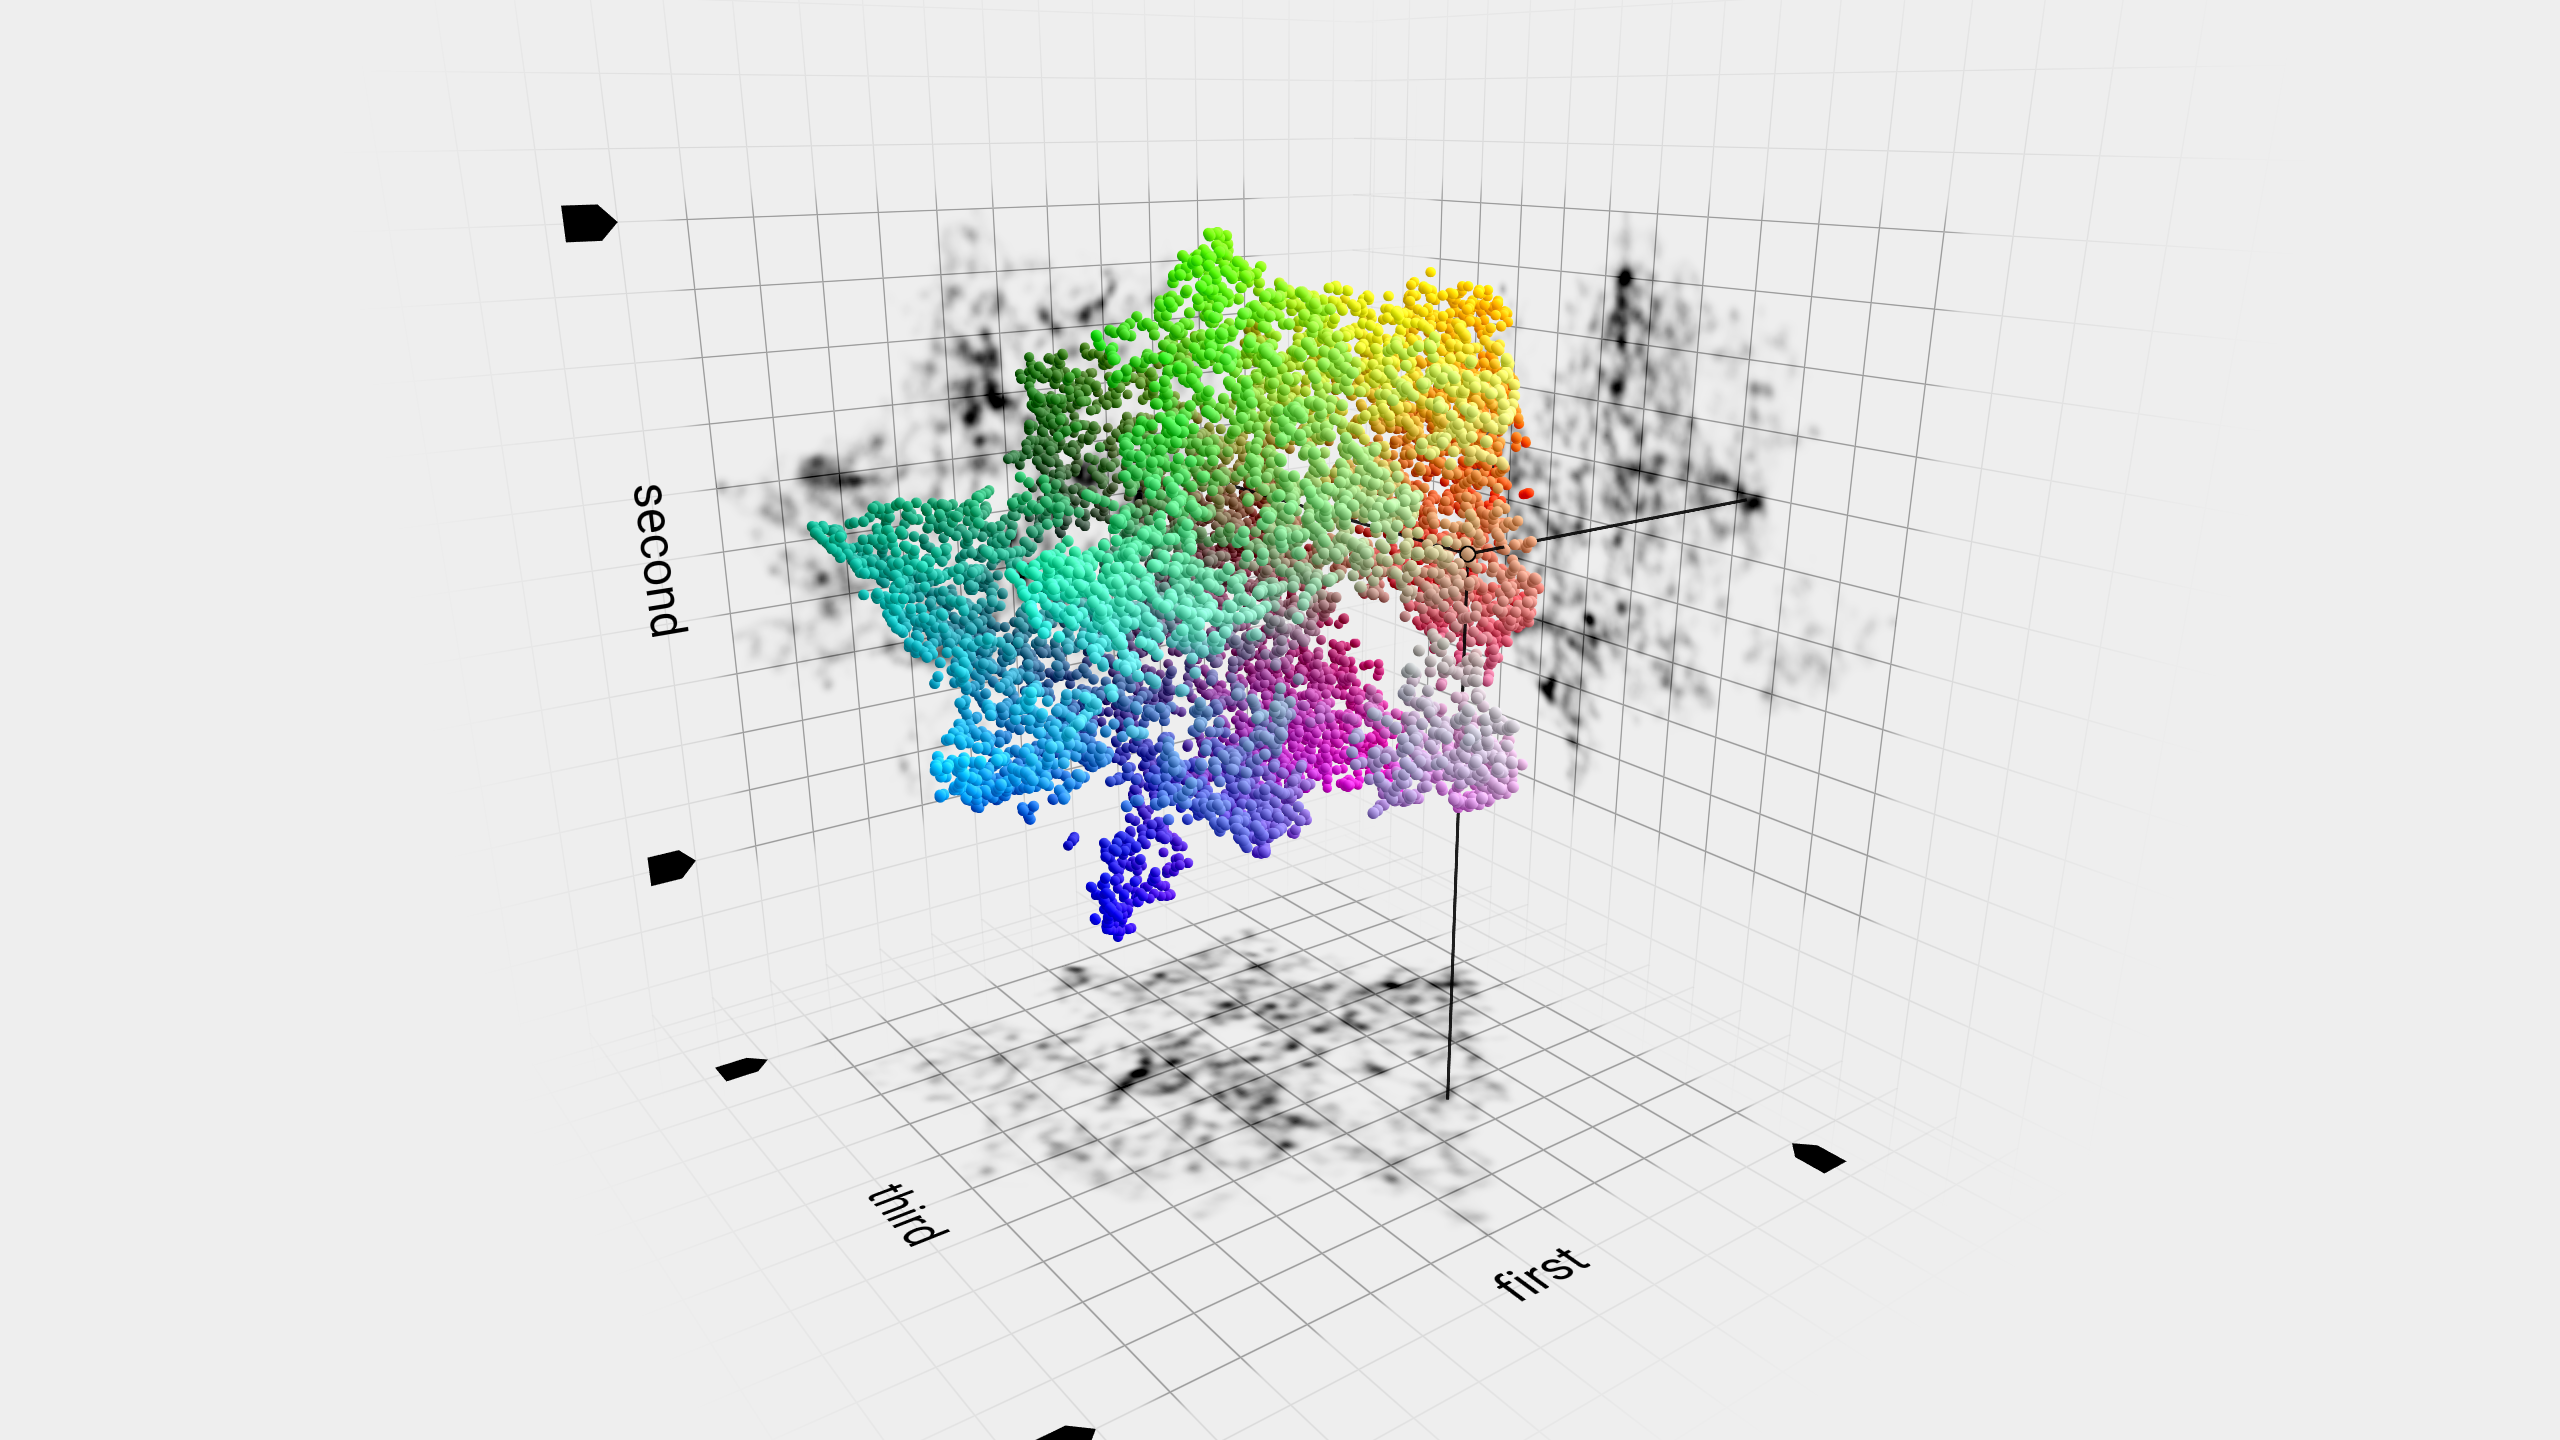
\includegraphics[width=\linewidth,trim={610 300 610 128},clip]{figures/teaser_v2.png}
        };
        \spy[white,spy connection path={\draw[thick] (tikzspyonnode) -- (tikzspyinnode);}] on ($(fig0.center)+(+12mm, +5mm)$) in node at ($(fig0.center)+(-30mm,-19.5mm)$);
        \spy[white,spy connection path={\draw[thick] (tikzspyonnode) -- (tikzspyinnode);}] on ($(fig0.center)+(+30mm, +8.5mm)$) in node at ($(fig0.center)+(+30mm,-19.5mm)$);
    \end{tikzpicture}
    \caption{%
        Example for the interactive exploration of a single data point. 
        The perpendicular lines provide a reference to all three 2D plots.}
    \label{fig:teaser_left}
  \end{subfigure}
  \hfill
  \begin{subfigure}[t]{0.49\linewidth}
    \centering
    \tikzsetnextfilename{teaser-2}
    \begin{tikzpicture}[figNS, spy using outlines = {magnification = 3.5, size = 22mm, connect spies,every spy on node/.append style={thick}}]
        \node[anchor = east](fig0) at (0,0)
        {
            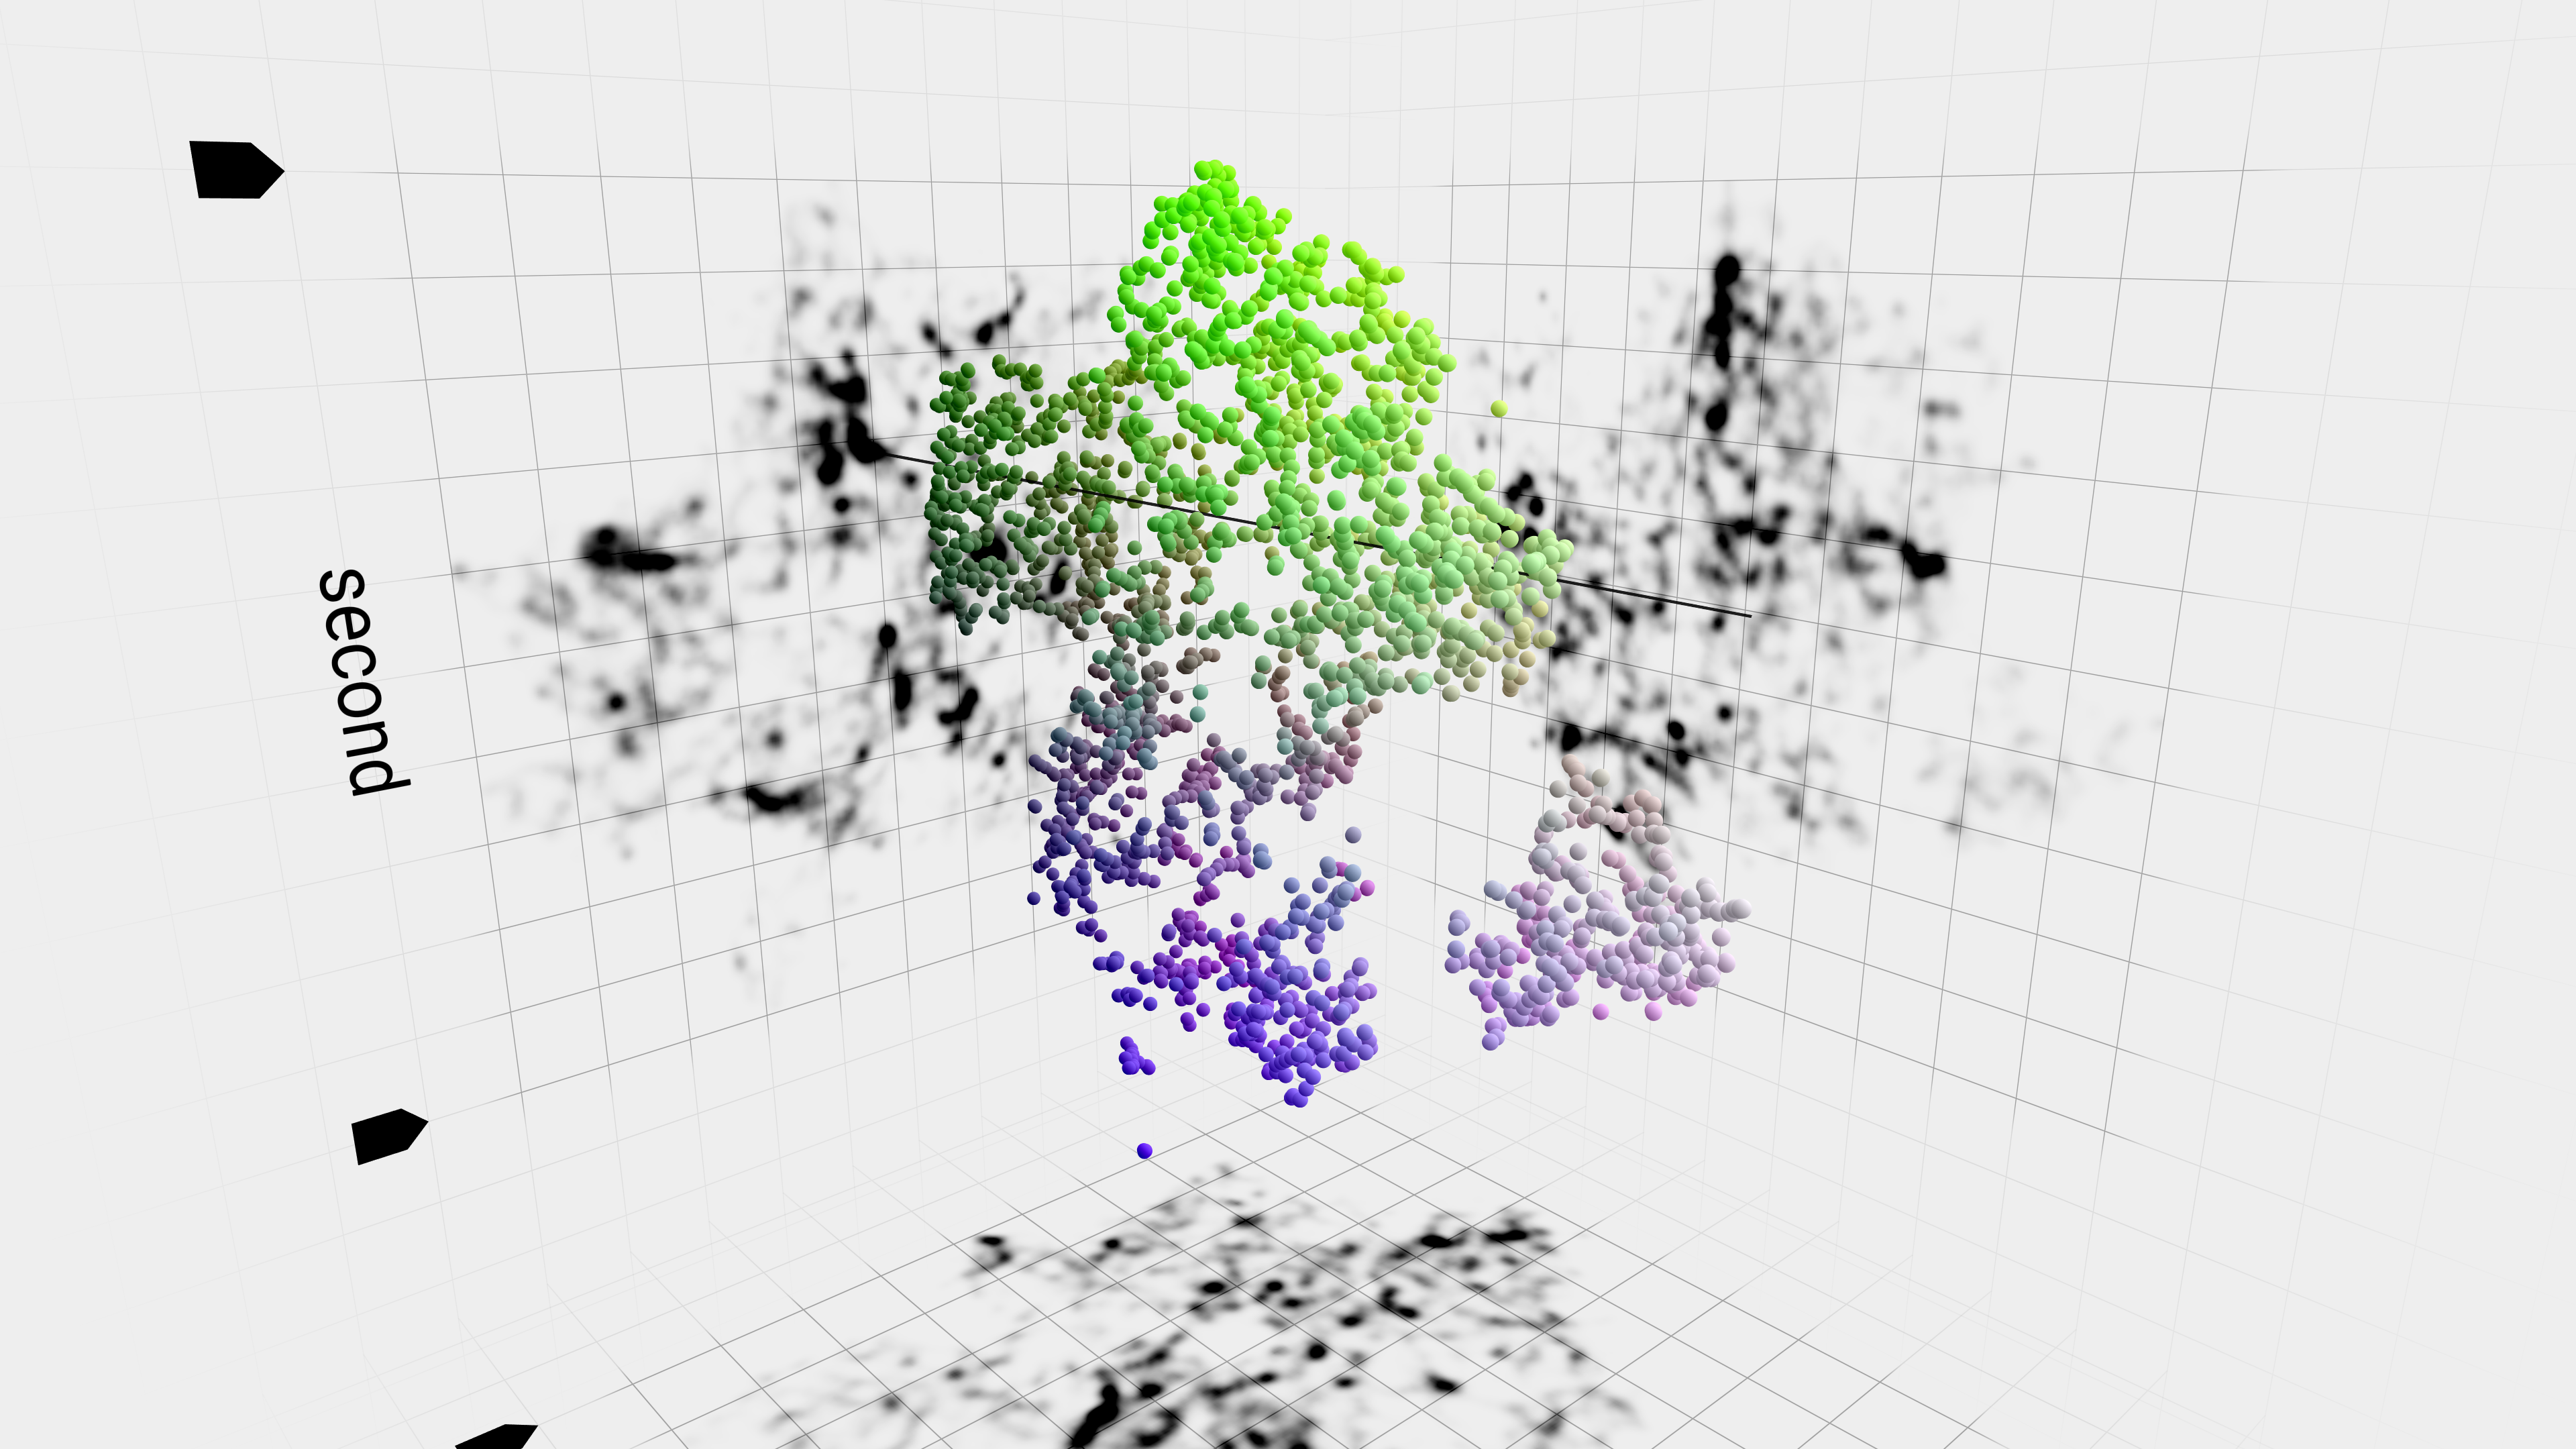
\includegraphics[width=\linewidth,trim={915 450 915 192},clip]{figures/teaser_plane2points.png}
        };
        \spy[white,spy connection path={\draw[thick] (tikzspyonnode) -- (tikzspyinnode);}] on ($(fig0.center)+(-26mm, +11.5mm)$) in node at ($(fig0.center)+(-30mm,-19.5mm)$);
        \spy[white,spy connection path={\draw[thick] (tikzspyonnode) -- (tikzspyinnode);}] on ($(fig0.center)+(-6mm, +8.5mm)$) in node at ($(fig0.center)+(+30mm,-19.5mm)$);
    \end{tikzpicture}
    \caption{%
        Example for the exploration of a dense area. 
        The line is perpendicular to the density map, referencing points within the 3D plot.}
    \label{fig:teaser_right}
  \end{subfigure}
  \vspace{-0.5\baselineskip}
  \caption{Two examples of datasets, explored using guides that link the 3D scatterplot to orthographic density maps.}
  \label{fig:teaser}
\end{teaserfigure}

\maketitle

\section{Introduction}
\label{sec:intro}
Scatter plots are commonly used to visualize and analyze relational as well as multivariate data sets.
Due to their ease of use and flexibility over data characteristics, they find use in countless domains and variations \cite{scatterplotSurvey,spDimRedChoices}.
The assignment of three scalar variables to the three main axes enables visual exploration of data in 3D.
However, as the number of data elements increases, 3D scatter plots increasingly suffer from occlusion.
To reduce its negative impact on exploration, the plot can be augmented by a scatter plot matrix.  

This paper extends the embedding of a scatter plot matrix into a 3D scatter plot, facilitating the exploration of the density and structure of the depicted data.
By providing the user with density plots representing x-ray-like perspectives within the 3D scatter plot, areas of interest become more discernible.
We provide interaction techniques that allow filtering out data points associated with a cluster.
Our web-based viewer uses WebGL~2 and allows for interactive analysis of multi-million point data sets.
It is free to use, hosted on
\href{https://varg.dev}{varg.dev}%
\footnote{\href{https://demo.varg.dev/vidi/web3d-2022}{demo.varg.dev/vidi/web3d-2022}}, 
and its source code is published on Github%
\footnote{\href{https://github.com/lukaswagner/vidi}{github.com/lukaswagner/vidi}}.
We complement this by discussing relevant API restrictions, storage limitations, and overall computational performance.

\section{Related Work}
Occlusion and overplotting are well-known issues for 3D and 2D scatterplots, respectively, and continue to be discussed in the field of (interactive) visualization \cite{occlusionTaxonomy}.
The majority of data elements within massive data sets displayed by a 3D scatter plot will be hidden behind or even surrounded on all sides by other data elements.
In the following, we provide a brief overview of common mitigation strategies such as highlighting planes, illustrative shadows, aggregation, and clustering.

One basic approach is to use 3D cutting planes, which hide all objects that fall on one side.
Placing the cutting planes requires knowledge about any data of interest being occluded by other data.
A variant of this approach are highlight planes, which reduce the scene elements to those close to a user-defined plane \cite{highlightPlane}.
Illustrative shadows address occlusion by embedding an additional view of the observed object into the scene \cite{illustrativeShadows}.
This approach projects the model onto a 2D plane.
Objects of interest are highlighted using non-photorealistic rendering.

Another approach for reducing occlusion issues is the reduction of scene elements.
For exploring large data sets, clustering allows gaining a overview over the data set by reducing the number of visible elements.
Rendering clusters as solid meshes instead of scatter plots \enquote{makes [\ldots] use of the innate 3D scene understanding capabilities of the human visual system} \cite{subspaceShapes}.
Splatterplots is an aggregation approach dedicated to scatter plots \cite{splatterplots}.
Instead of clustering, a less computation-heavy approach is binning.
Typically, the data points are grouped into hyperrectangles, however, other patterns can be used as well \cite{binning}.
Alternatively to single-level aggregation, it's also possible to use hierarchical aggregations \cite{hierarchAggr}.
This has the advantage of providing multiple layers of abstraction.
Instead of reducing visible data points using aggregation, the points can also be filtered by some metric.
Building on Splatterplots, it is possible to filter the data points to represent the splats \cite{spSmartFilter}.

Another challenge for 3D scatter plots is spatial perception.
There are different approaches to improving readability.
A natural first approach is the addition of shading.
One possible option is cushion shading, which utilizes the fragment position to efficiently approximate realistic shading \cite{cushionShading}.
Improving over this, ambient occlusion provides visual hints about spatial relations.
For scatter plots, specific point-based ambient occlusion algorithms exist \cite{pointAO}.
Furthermore, the restrictions of a 2D screen can be circumvented by using virtual reality headset or similar 3D technologies.
All of these, however, do not solve the occlusion issues.

A possible solution for occlusion in 3D scatter plots are scatter plots matrices.
Scatter plot matrices can also be used to navigate high-dimensional data sets \cite{scatplotnav}.
The typical 2D matrix approach, however, does not provide much in the way of discovering the relationships between the graphs.
For three dimensions, this can be improved by placing these graphs orthogonal to the three main axes.
This adapts the scatter plot matrix, which is purely juxtapositional, into a combination of compositions \cite{compositeVis}:
The 2D plots are nested into the 3D scene.
Visually, however, the 2D plots are either juxtaposed or superimposed with the 3D plot, based on the viewing angle.
Such an integration of 2D scatter plots is already supported in some 3D scatter plot viewers.
One variant of this are Regression Cubes, especially when examining both a 3D view and the three axis-aligned 2D facets \cite{regrCubes}.
In sufficiently complex scenes, however, the 2D scatter plots may suffer from over-plotting, in turn hindering insights into the 3D visualization.

One approach to solving over-plotting issues is reducing the opacity of the rendered points, e.g. by dynamically selecting an opacity based on the local density of points \cite{dynOpacity2dSP}.
Apart from opacity, other design parameters, such as the point size, can be automatically adjusted as well \cite{spPerceptOpti}.
It is also possible to provide the user with more detailed views of high-density areas \cite{nestedSP}.
In order to improve readability of 2D scatter plots, it's also possible to smooth out the plotted data using statistical metrics \cite{spSmoothing}.
This results in minor details being dropped, letting the user focus on the data set's macro-structure.

\section{Visualization Design}
\label{sec:design}

The data set displayed by a 3D scatter plot is contained in an axis-aligned bounding box.
Typically, the six bounding planes provide the user with a grid for orientation.
They can be used as billboards that visualize additional information.
We use an orthographic projection to plot the data on these bounding planes.
As known from architectural drawings, the resulting 2D scatter plots are comparable to the ground plan, front elevation, and side elevation.
These views represent the different panes of a scatter plot matrix.

In order to eliminate the over-plotting we propose creating density maps instead of simple 2D scatter plots.
Thereby, more than one data point can affect the resulting scatter plot at any rasterized location.
When plotting the data points, we render a gradient, starting with the maximum density at the point's center and falling off with increasing distance.
By additively blending all points, we obtain an image where each pixel contains information about how many points are close to it.
The density maps are then be projected onto the 3D scatter plot's grids, as shown in \autoref{fig:clusters}.
This allows the user to spot and locate clusters of data points which may be occluded and concealed otherwise.

\begin{figure}
  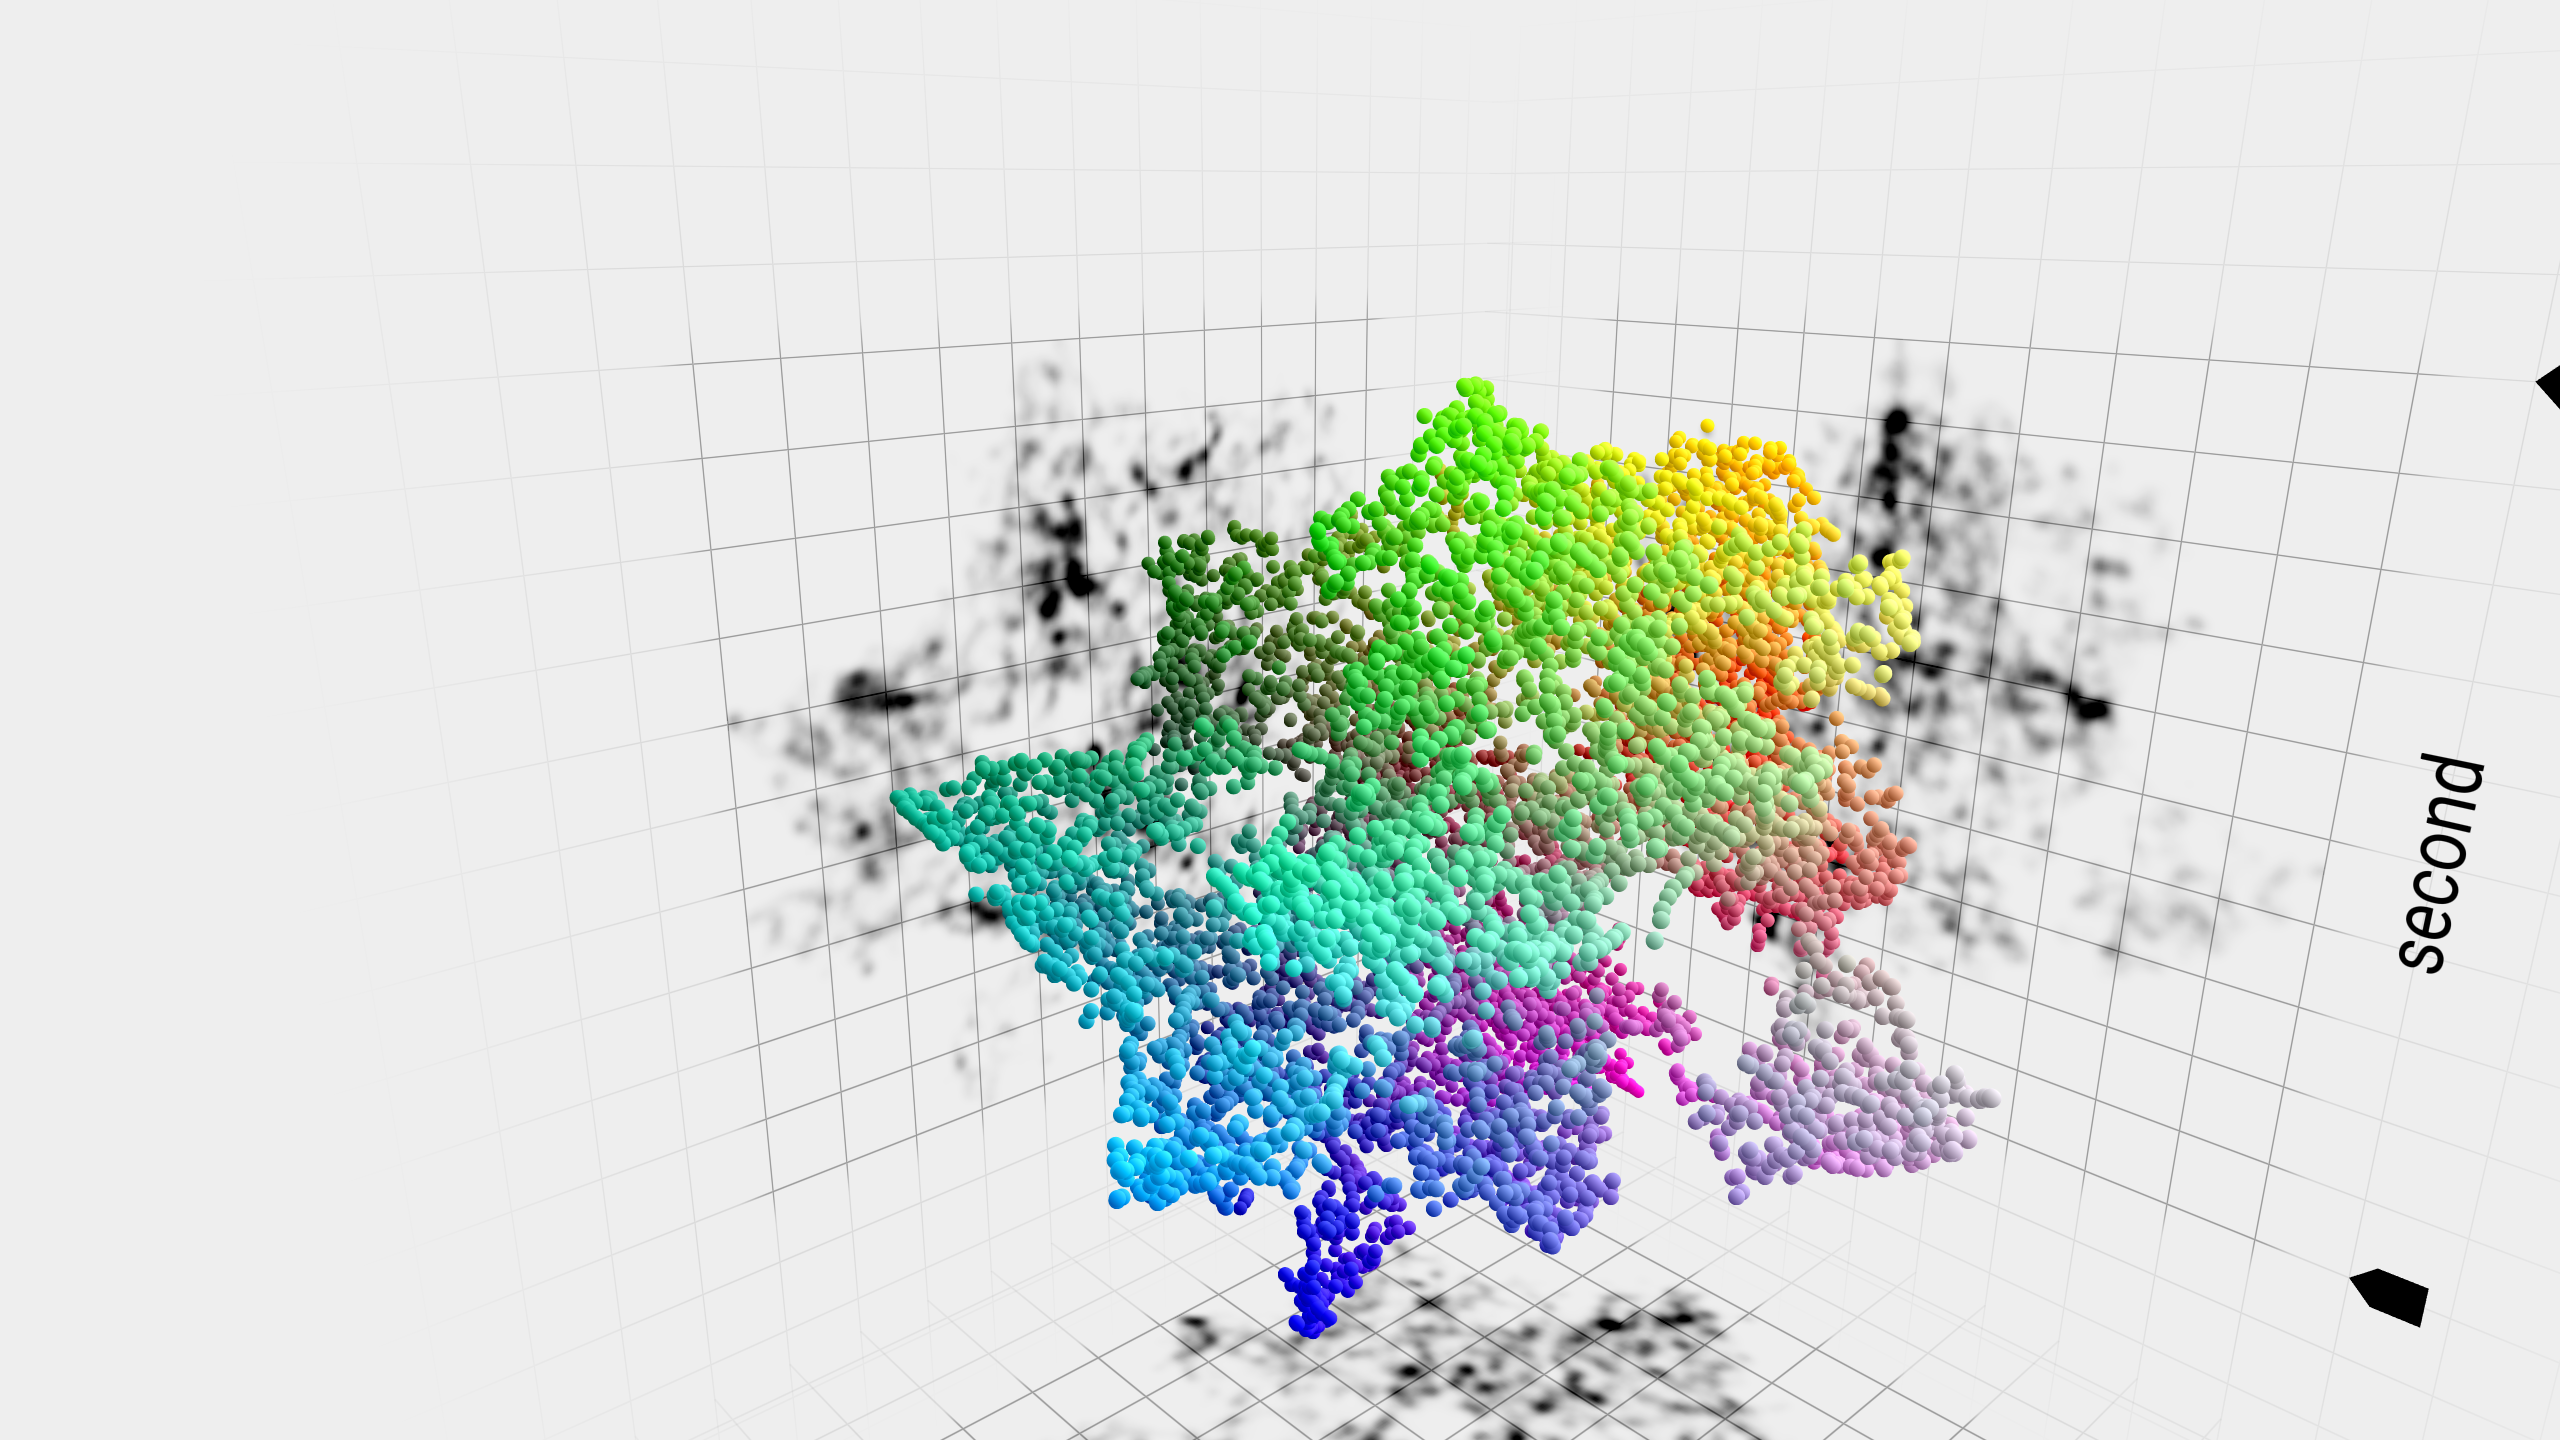
\includegraphics[width=\linewidth,trim={30cm 22cm 32cm 15cm},clip]{figures/clusters_v2.png}
  \vspace{-1.0\baselineskip}
  \caption{Additive blending of graphical elements into a density map reveals data clusters.}
  \label{fig:clusters}
\end{figure}

We map the intensity to a color scale to improve its readability.
\autoref{fig:colors} gives an overview of example color schemes.
While different color schemes do not change the actual data being displayed, they can help by increasing the output resolution and connecting the data to more accustomed concepts.
Alternatively, we can reduce the resolution of the color scale which results in more discernible color bands that denote areas of equal density (contour intervals).

\begin{figure}[t]
  \centering
  \begin{subfigure}[t]{0.32\linewidth}
    \centering
    \tikzsetnextfilename{inferno-c}
    \begin{tikzpicture}[inner sep=0pt,outer sep=0pt]
        \node[] (image) { 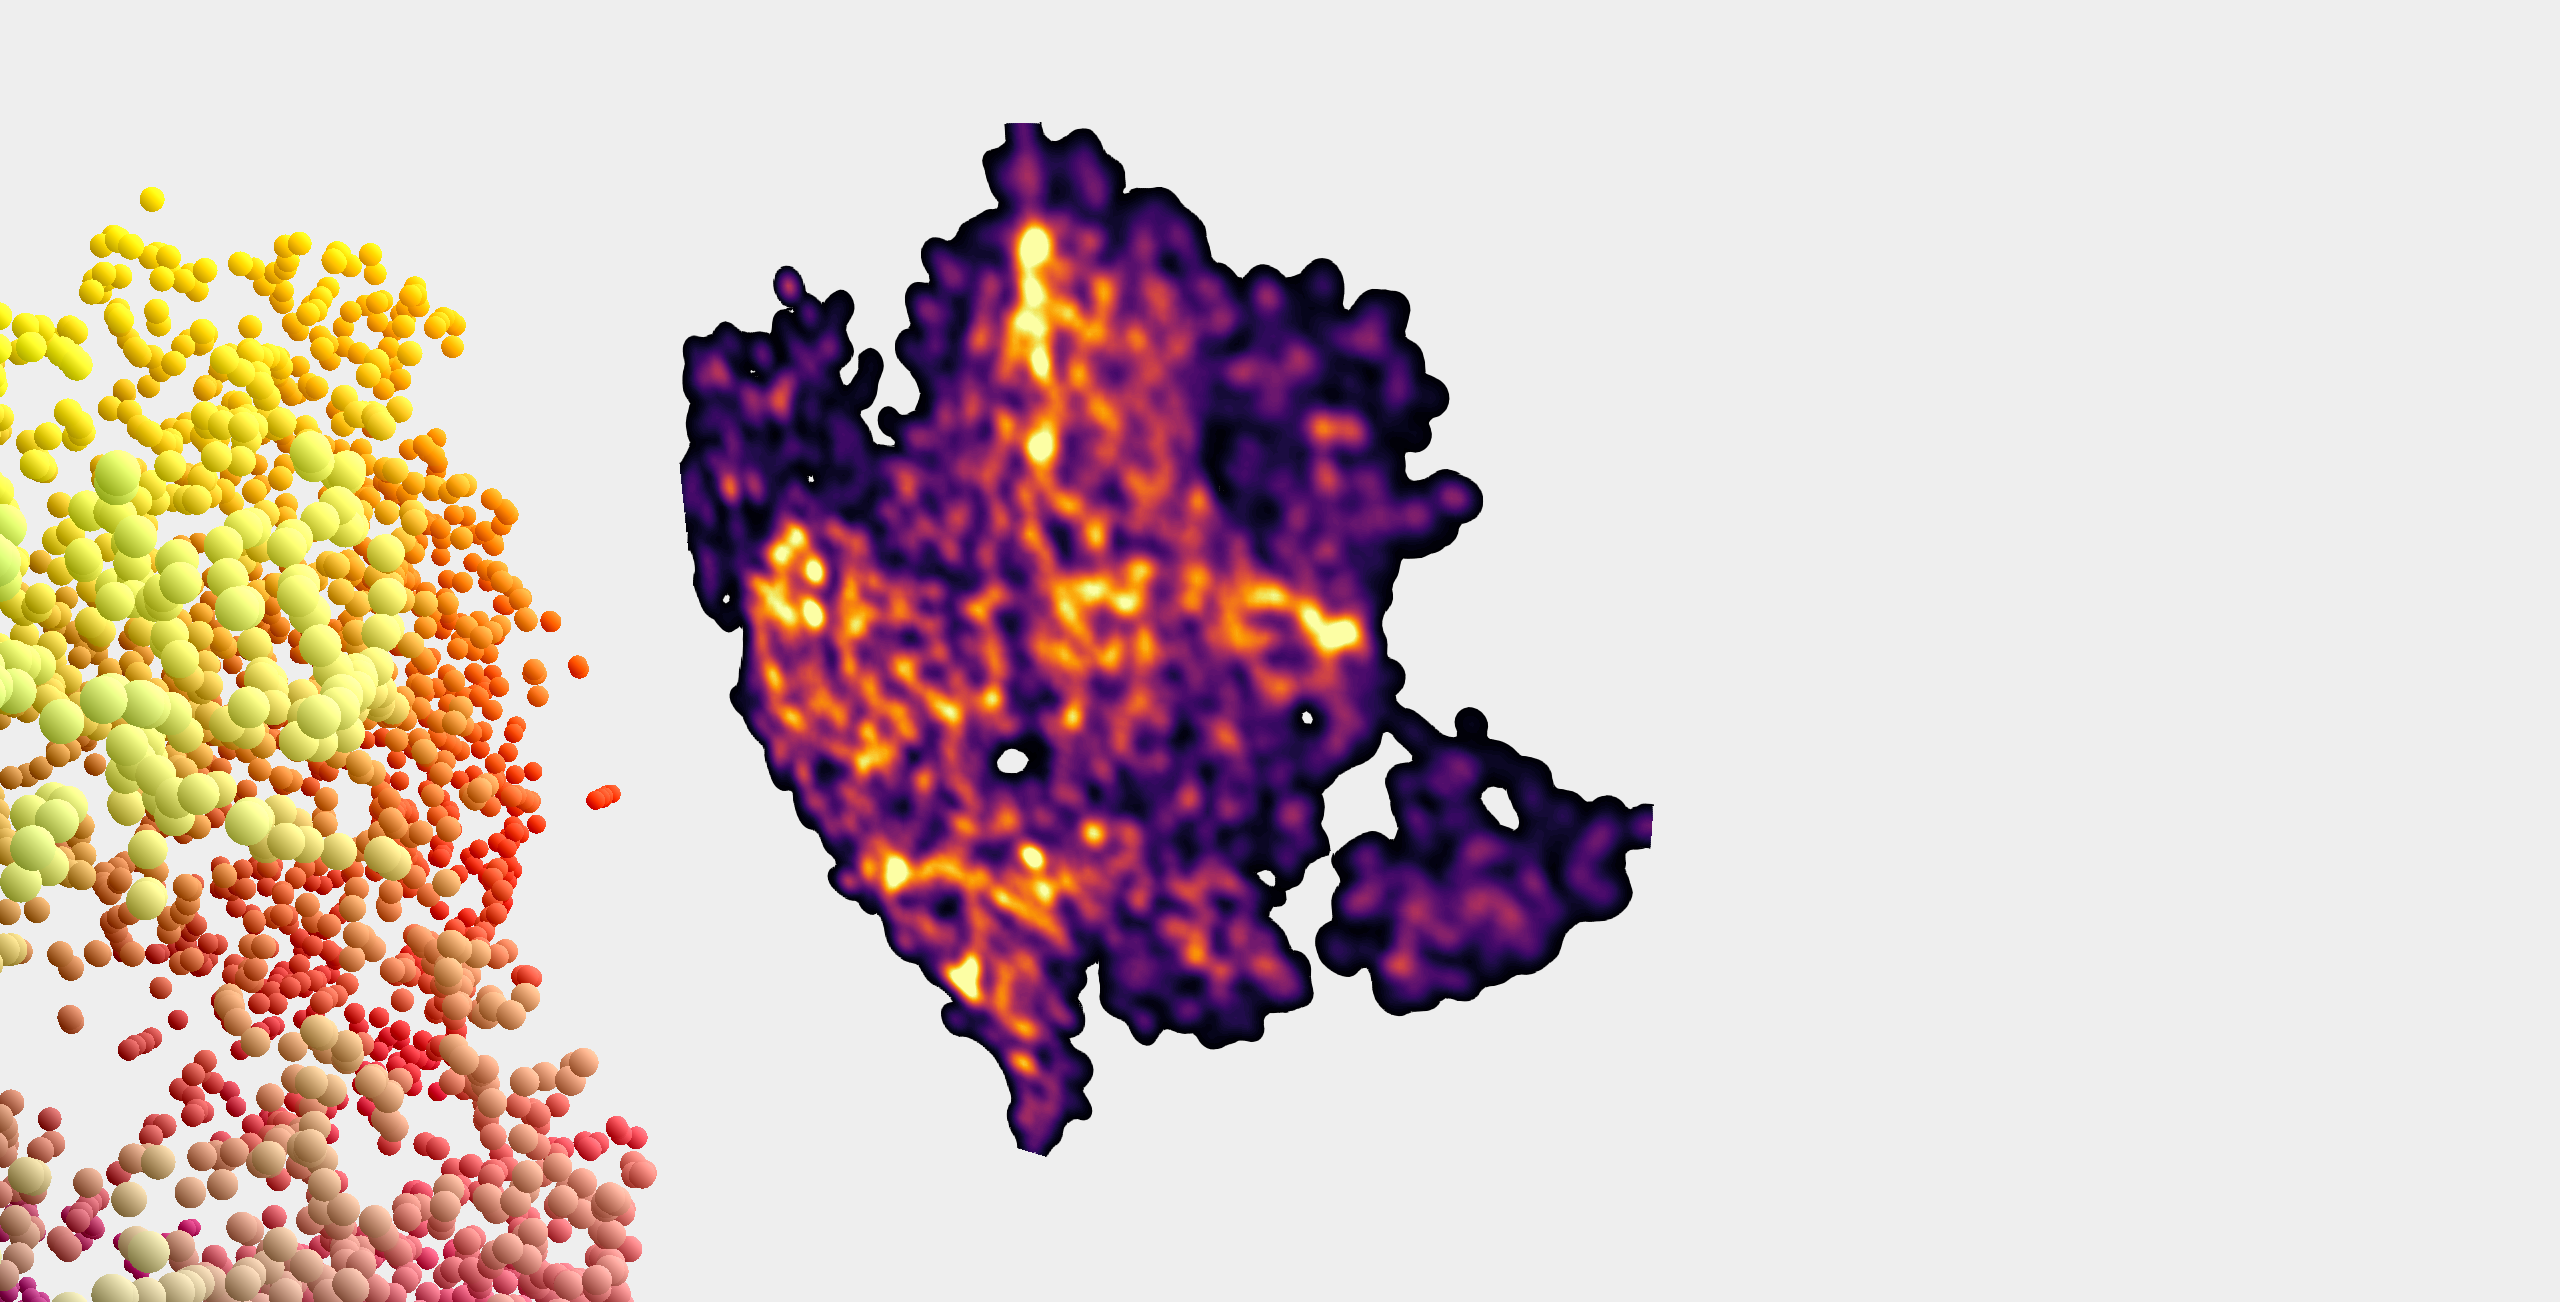
\includegraphics[width=0.92\linewidth,trim={30cm 28cm 45cm 7cm},clip]{figures/color_inferno.png} };
        \gettikzxy{(image.north)}{\nx}{\ny}
        \gettikzxy{(image.south)}{\sx}{\sy}
        \pgfmathparse{\ny-\sy}
        \pgfmathsetmacro{\imageheight}{\pgfmathresult}
        \begin{axis}[
            at={($(image.south east)+(1pt,0pt)$)},
            hide axis,
            scale only axis,
            height=0cm,
            width=0cm,
            colormap/inferno64,
            colorbar horizontal,
            point meta min=0,
            point meta max=0,
            colorbar style={
                axis line style = { draw = none },
                width=\imageheight pt,
                height=0.04\linewidth,
                rotate=90,
                xtick style={draw=none},
                point meta min=0,
                point meta max=1000,
                xticklabels={},
                xticklabel style={},
                anchor=south west,
                at={(0,0)}
            }]
            \addplot [draw=none] coordinates {(0,0) (1,1)};
        \end{axis}
    \end{tikzpicture}
    \caption{Inferno}
    \label{fig:colorInferno}
  \end{subfigure}
  \hfill
  \begin{subfigure}[t]{0.32\linewidth}
    \centering
    \tikzsetnextfilename{spectral-64}
    \begin{tikzpicture}[inner sep=0pt,outer sep=0pt]
        \node[] (image) { 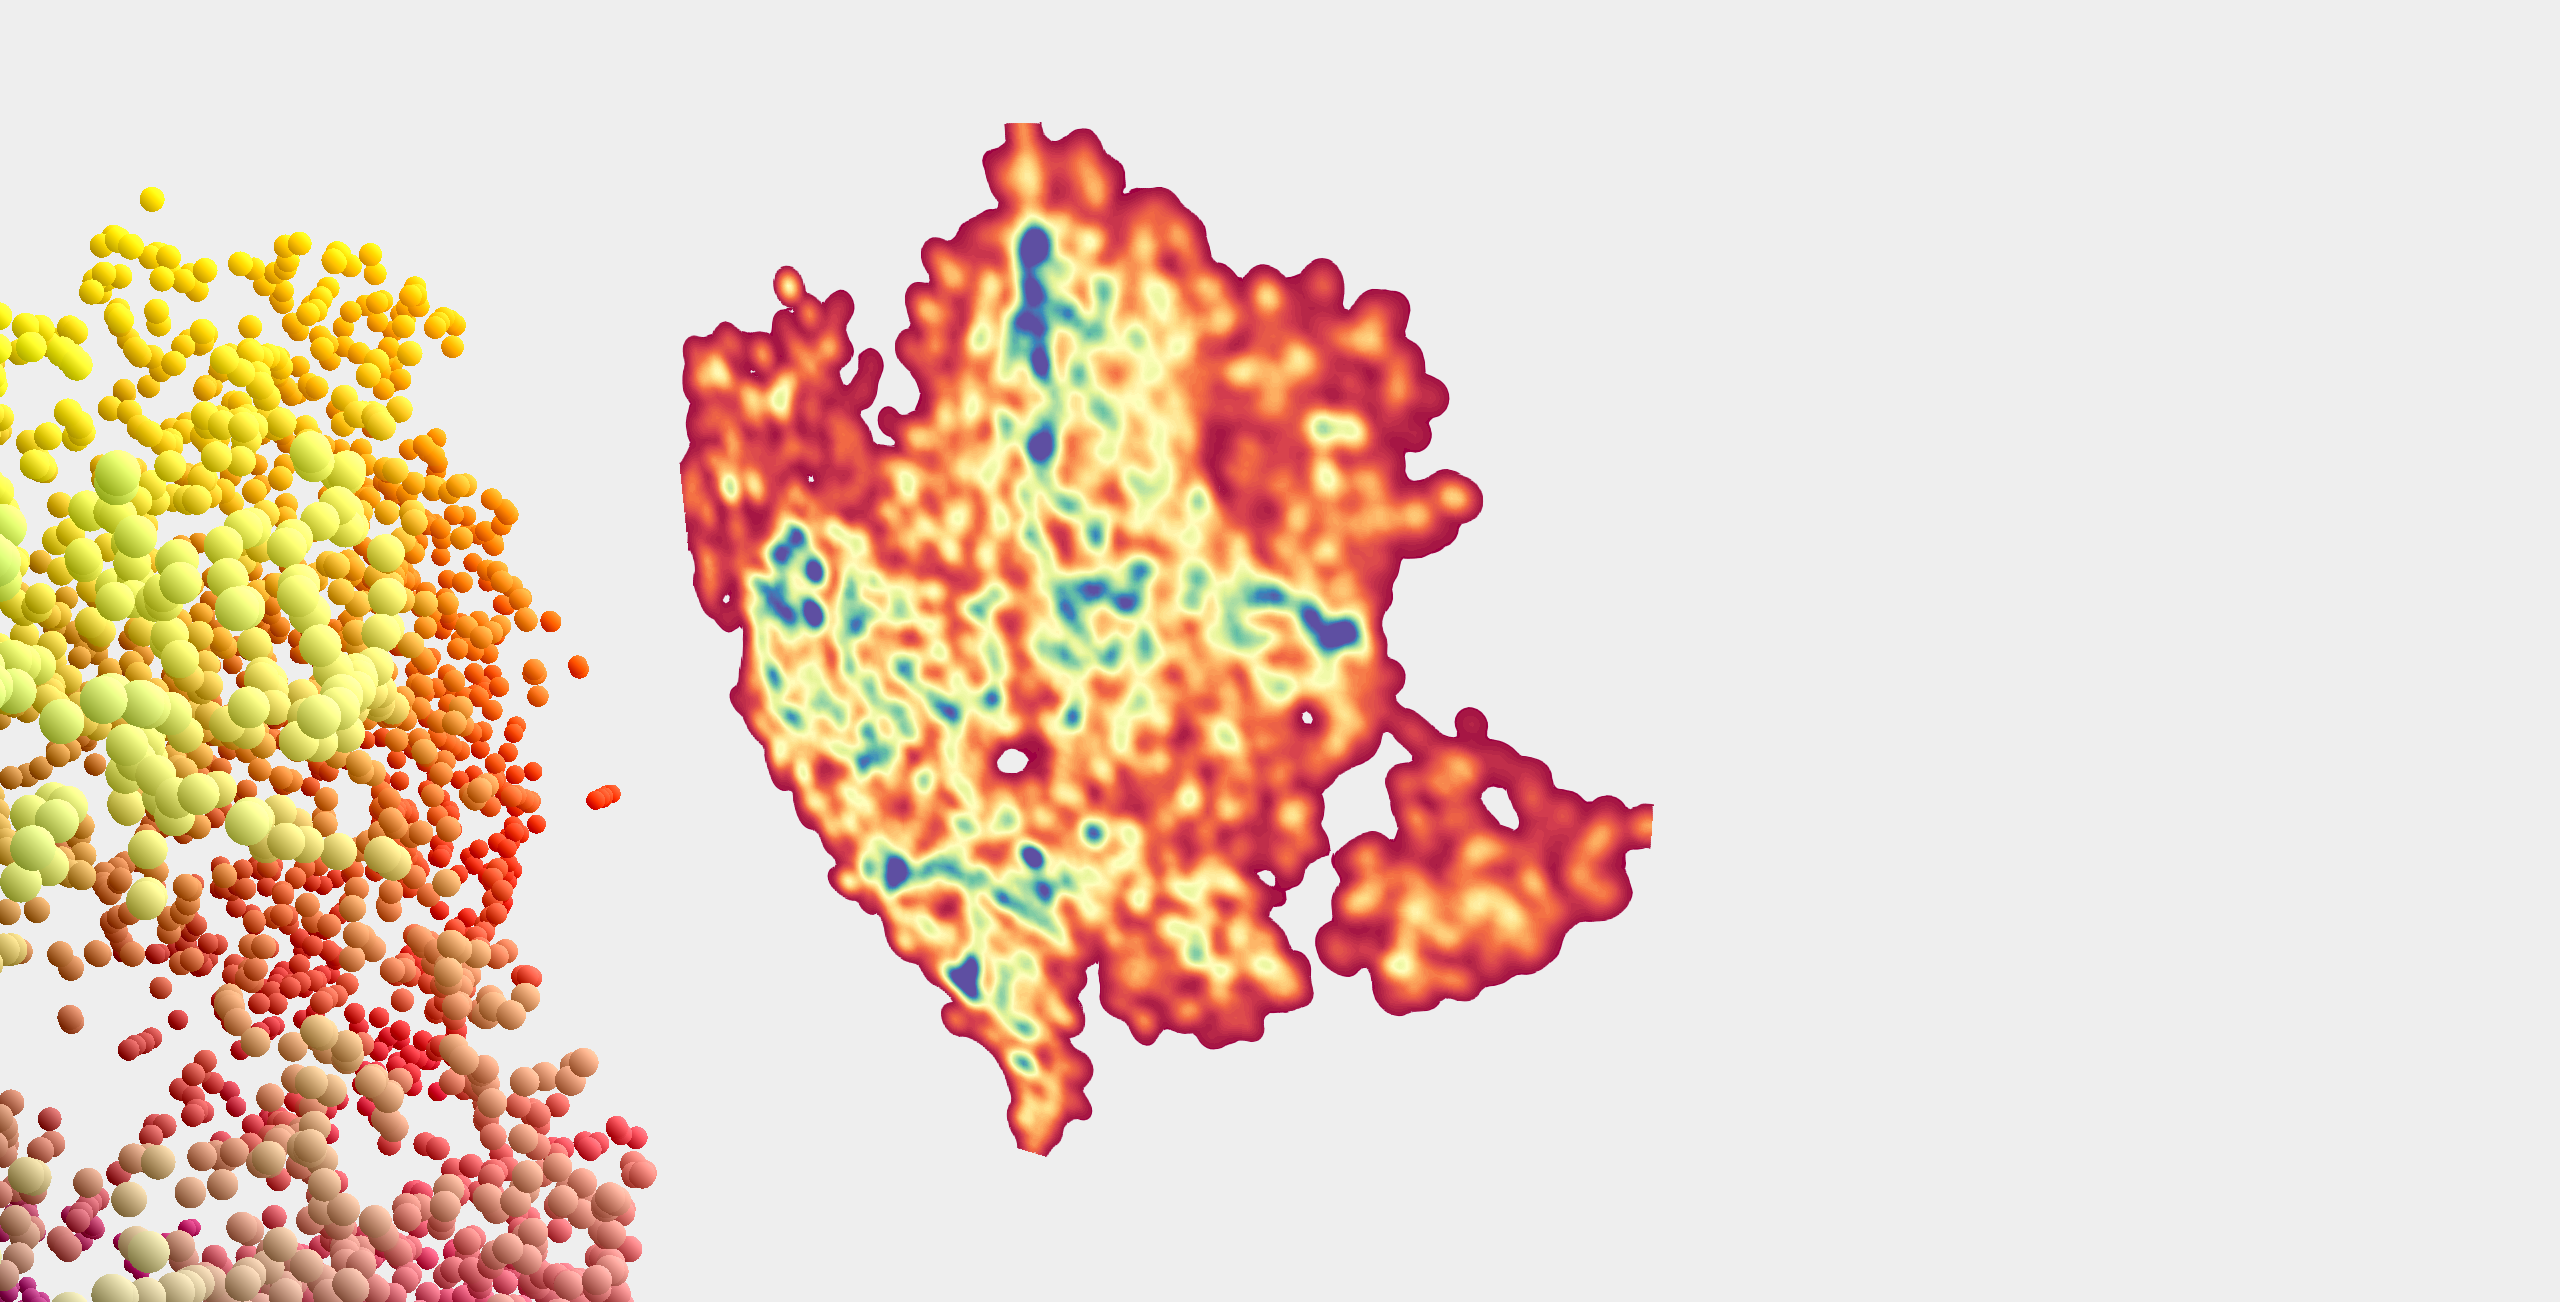
\includegraphics[width=0.92\linewidth,trim={30cm 28cm 45cm 7cm},clip]{figures/color_spectral_64.png} };
        \gettikzxy{(image.north)}{\nx}{\ny}
        \gettikzxy{(image.south)}{\sx}{\sy}
        \pgfmathparse{\ny-\sy}
        \pgfmathsetmacro{\imageheight}{\pgfmathresult}
        \begin{axis}[
            at={($(image.south east)+(1pt,0pt)$)},
            hide axis,
            scale only axis,
            height=0cm,
            width=0cm,
            colormap/spectral64,
            colorbar horizontal,
            point meta min=0,
            point meta max=0,
            colorbar style={
                axis line style = { draw = none },
                width=\imageheight pt,
                height=0.04\linewidth,
                rotate=90,
                xtick style={draw=none},
                point meta min=0,
                point meta max=1000,
                xticklabels={},
                xticklabel style={},
                anchor=south west,
                at={(0,0)}
            }]
            \addplot [draw=none] coordinates {(0,0) (1,1)};
        \end{axis}
    \end{tikzpicture}
    \caption{Spectral, 64 steps}
    \label{fig:colorSpectral64}
  \end{subfigure}
  \hfill
  \begin{subfigure}[t]{0.32\linewidth}
    \centering
    \tikzsetnextfilename{spectral-7}
    \begin{tikzpicture}[inner sep=0pt,outer sep=0pt]
        \node[] (image) { 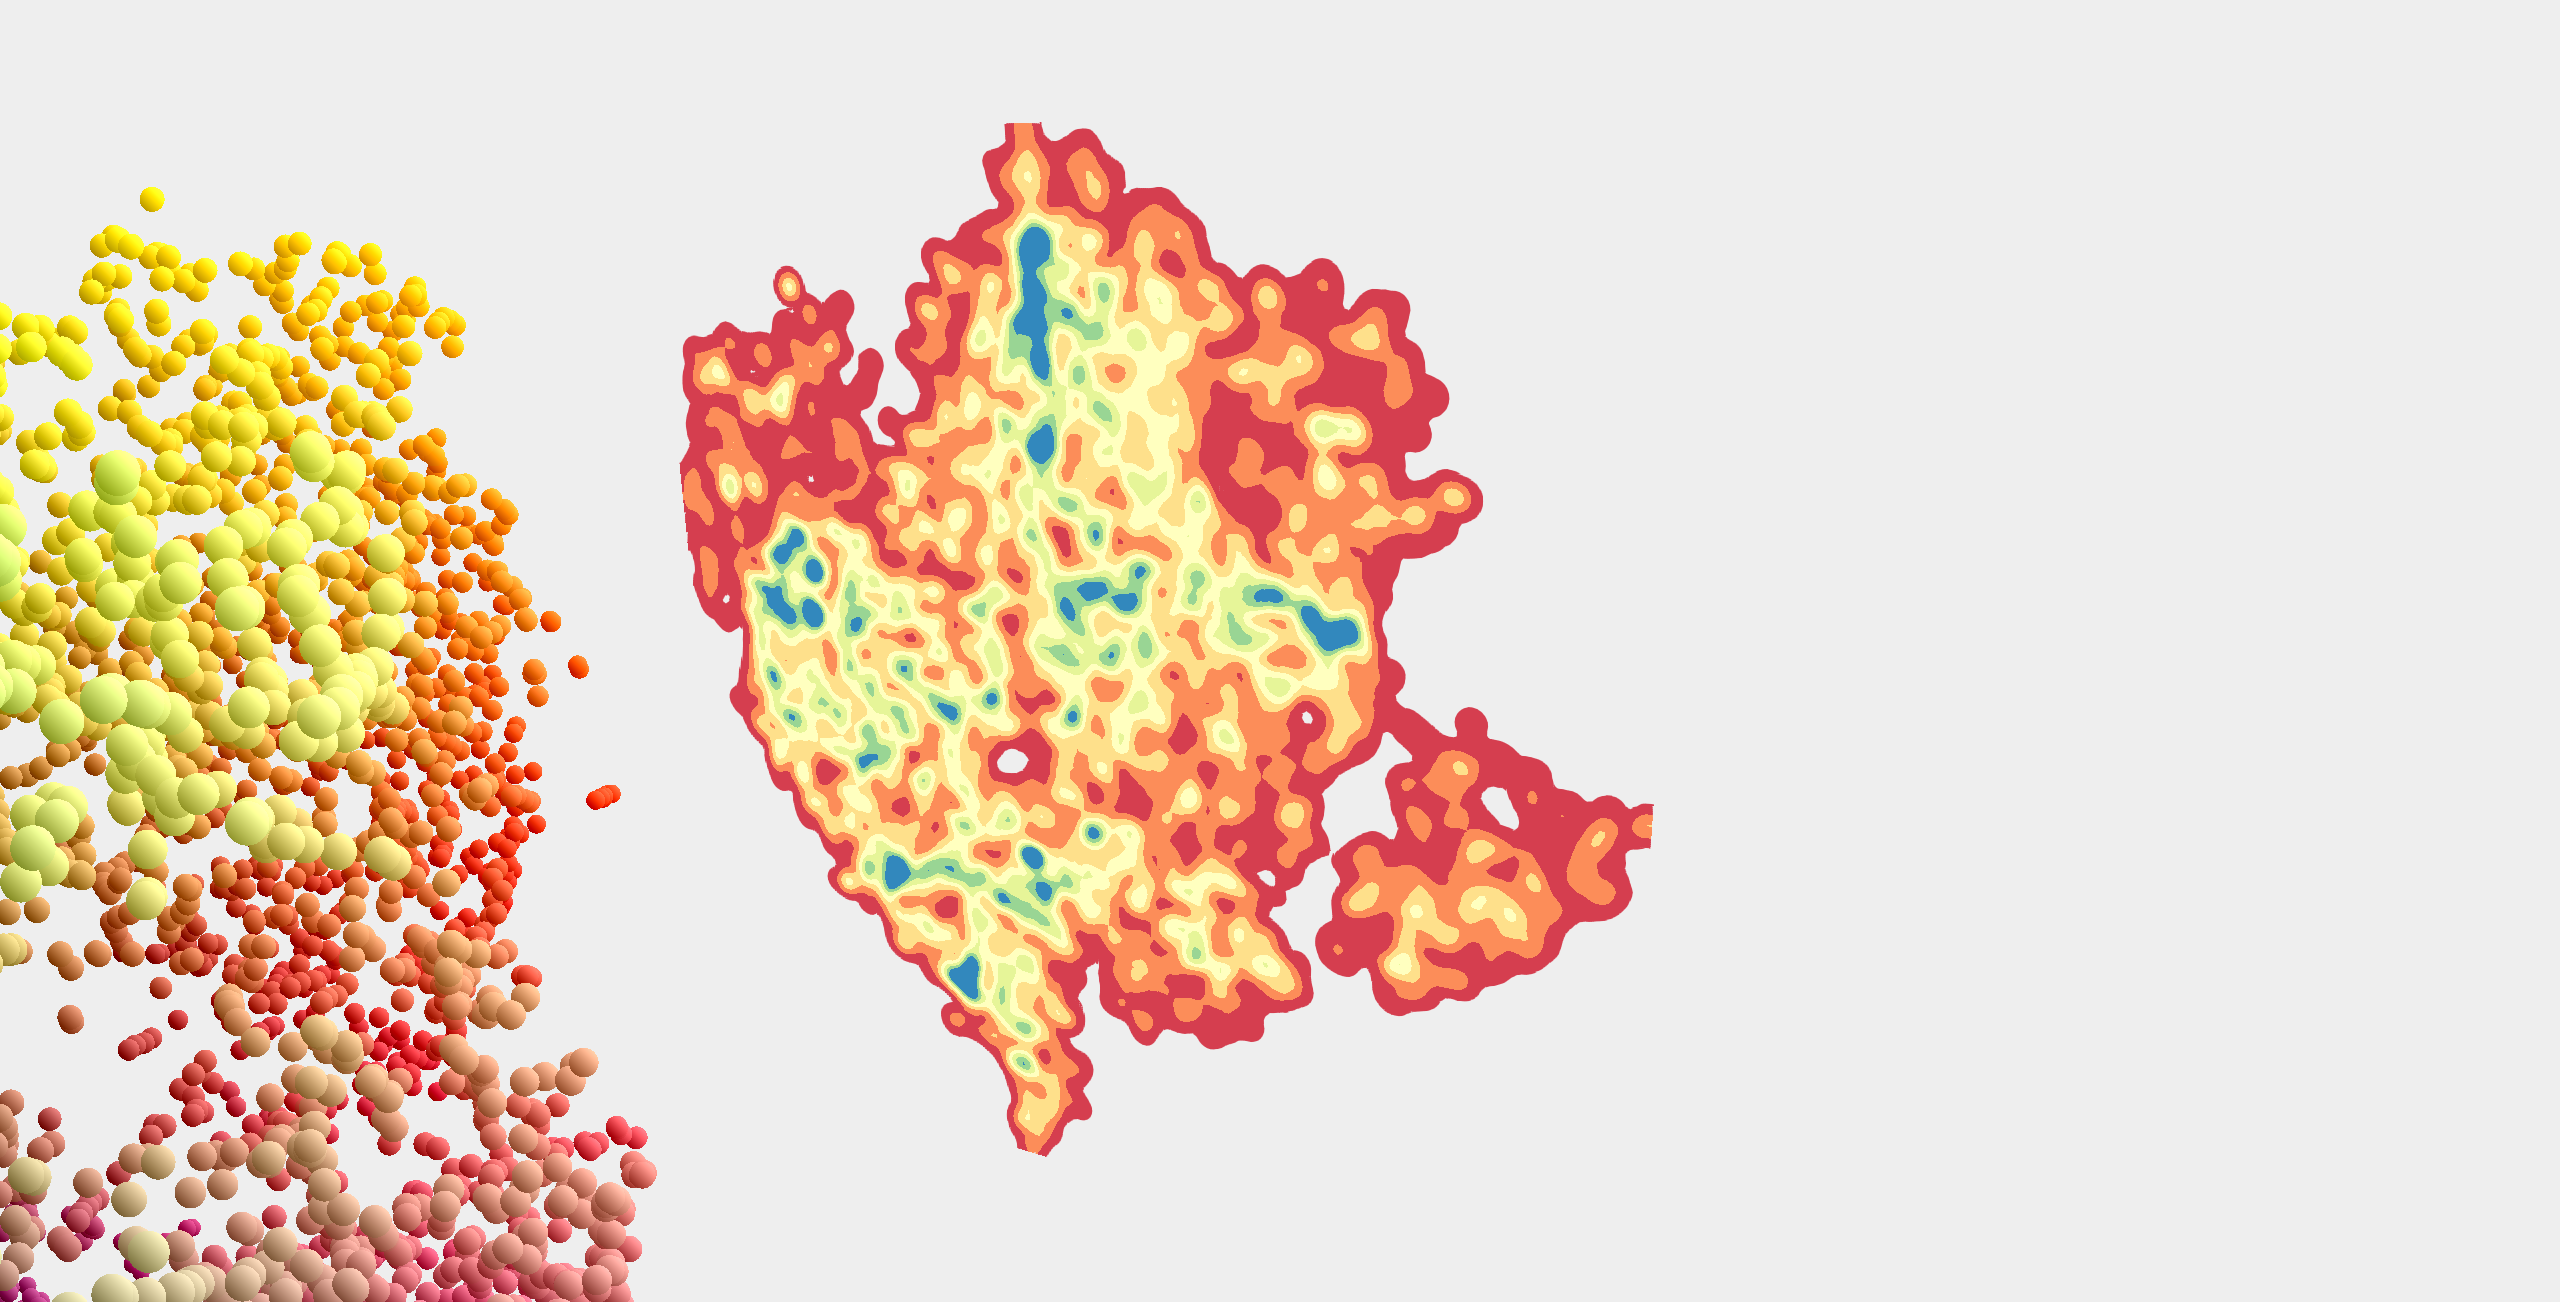
\includegraphics[width=0.92\linewidth,trim={30cm 28cm 45cm 7cm},clip]{figures/color_spectral_7.png} };
        \gettikzxy{(image.north)}{\nx}{\ny}
        \gettikzxy{(image.south)}{\sx}{\sy}
        \pgfmathparse{\ny-\sy}
        \pgfmathsetmacro{\imageheight}{\pgfmathresult}
        \begin{axis}[
            at={($(image.south east)+(1pt,0pt)$)},
            hide axis,
            scale only axis,
            height=0cm,
            width=0cm,
            colormap/spectral7,
            colorbar horizontal,
            colorbar as palette,
            colorbar style={
                axis line style = { draw = none },
                width=\imageheight pt,
                height=0.04\linewidth,
                rotate=90,
                xtick style={draw=none},
                point meta min=0,
                point meta max=7,
                xtick={},
                xticklabels={},
                xticklabel style={},
                anchor=south west,
                at={(0,0)}
            }]
            \addplot [draw=none] coordinates {(0,0) (1,1)};
        \end{axis}
    \end{tikzpicture}
    \caption{Spectral, 7 steps}
    \label{fig:colorSpectral7}
  \end{subfigure}
  \vspace{-0.5\baselineskip}
  \caption{The same density map rendered with different color schemes (\ref{fig:colorInferno} and \ref{fig:colorSpectral64}) and color resolutions (\ref{fig:colorSpectral64} and \ref{fig:colorSpectral7}).}
  \label{fig:colors}
\end{figure}

In order to increase the scatter plot's interactive capabilities, we use graphical control elements integrated within the 3D scene.
As the browser only provides interaction with HTML elements, this requires implementation of techniques such as picking (\autoref{sec:impl}).
The user might want to filter and locate data points belonging to certain areas within the density maps.
This is supported by hiding any data points occluding the area of interest.
For this use case, we provide the user with sliders controlling axis aligned cutting planes.
These controls are placed co-planar to the grids and density maps.
This allows using the grid lines as reference for placing the control handles based on the density maps.

Another challenge is deducting a 3D point's position on the 2D density maps.
When hovering the cursor over a data point, we provide the user with reference lines to the respective position on all three planes (\autoref{fig:refline}).
These reference lines are axis-aligned and thus perpendicular on the planes.
Inversely, we also provide the user with reference lines from a 2D map into the 3D scatter plot.
By clicking on any of the density maps, the user can place such a line.
This reference line once again is placed perpendicular on the respective plane (\autoref{fig:reflineGrid}).
Together, these reference line interaction techniques facilitate cross-references between the 3D scatter plot and the 2D density maps.

\begin{figure}
  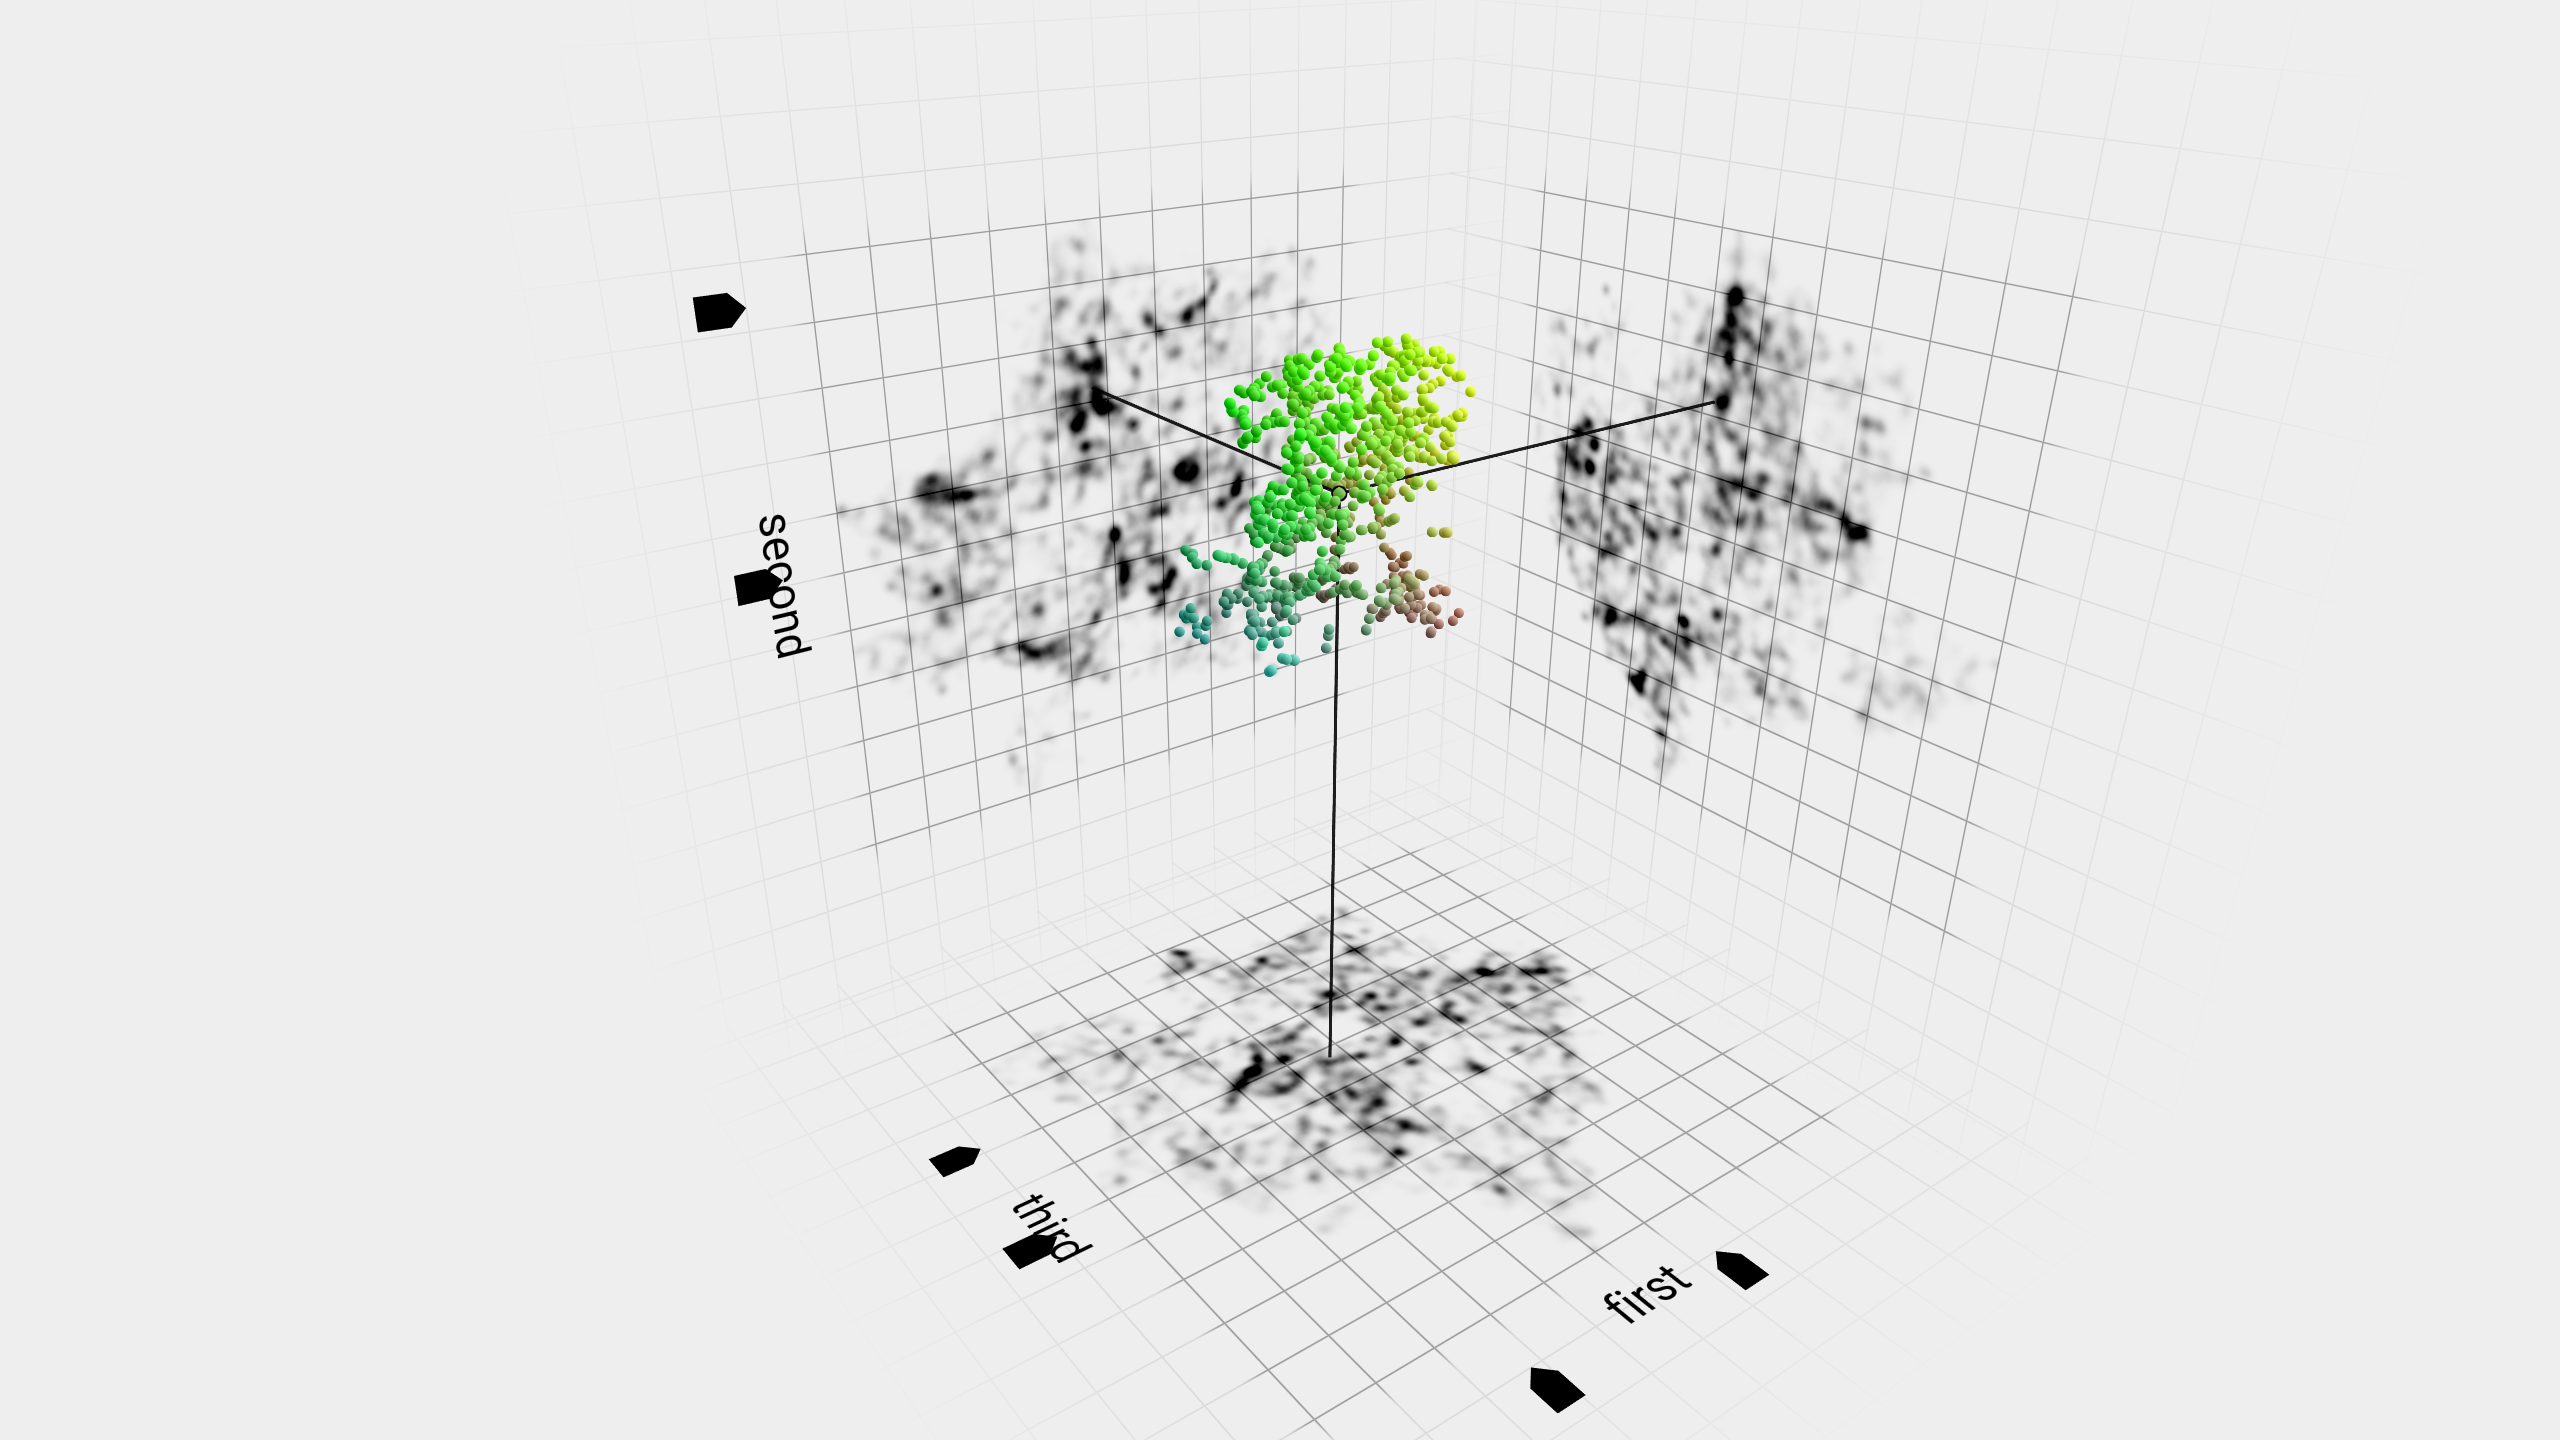
\includegraphics[width=\linewidth,trim={35cm 30cm 27cm 12cm},clip]{figures/refline_v2.png}
  \caption{Reference lines to all three planes provide easy evaluation of a point's position on the density maps. Here, the selected data point shares its position with many others on the right and left density maps.}
  \label{fig:refline}
\end{figure}

\begin{figure}
  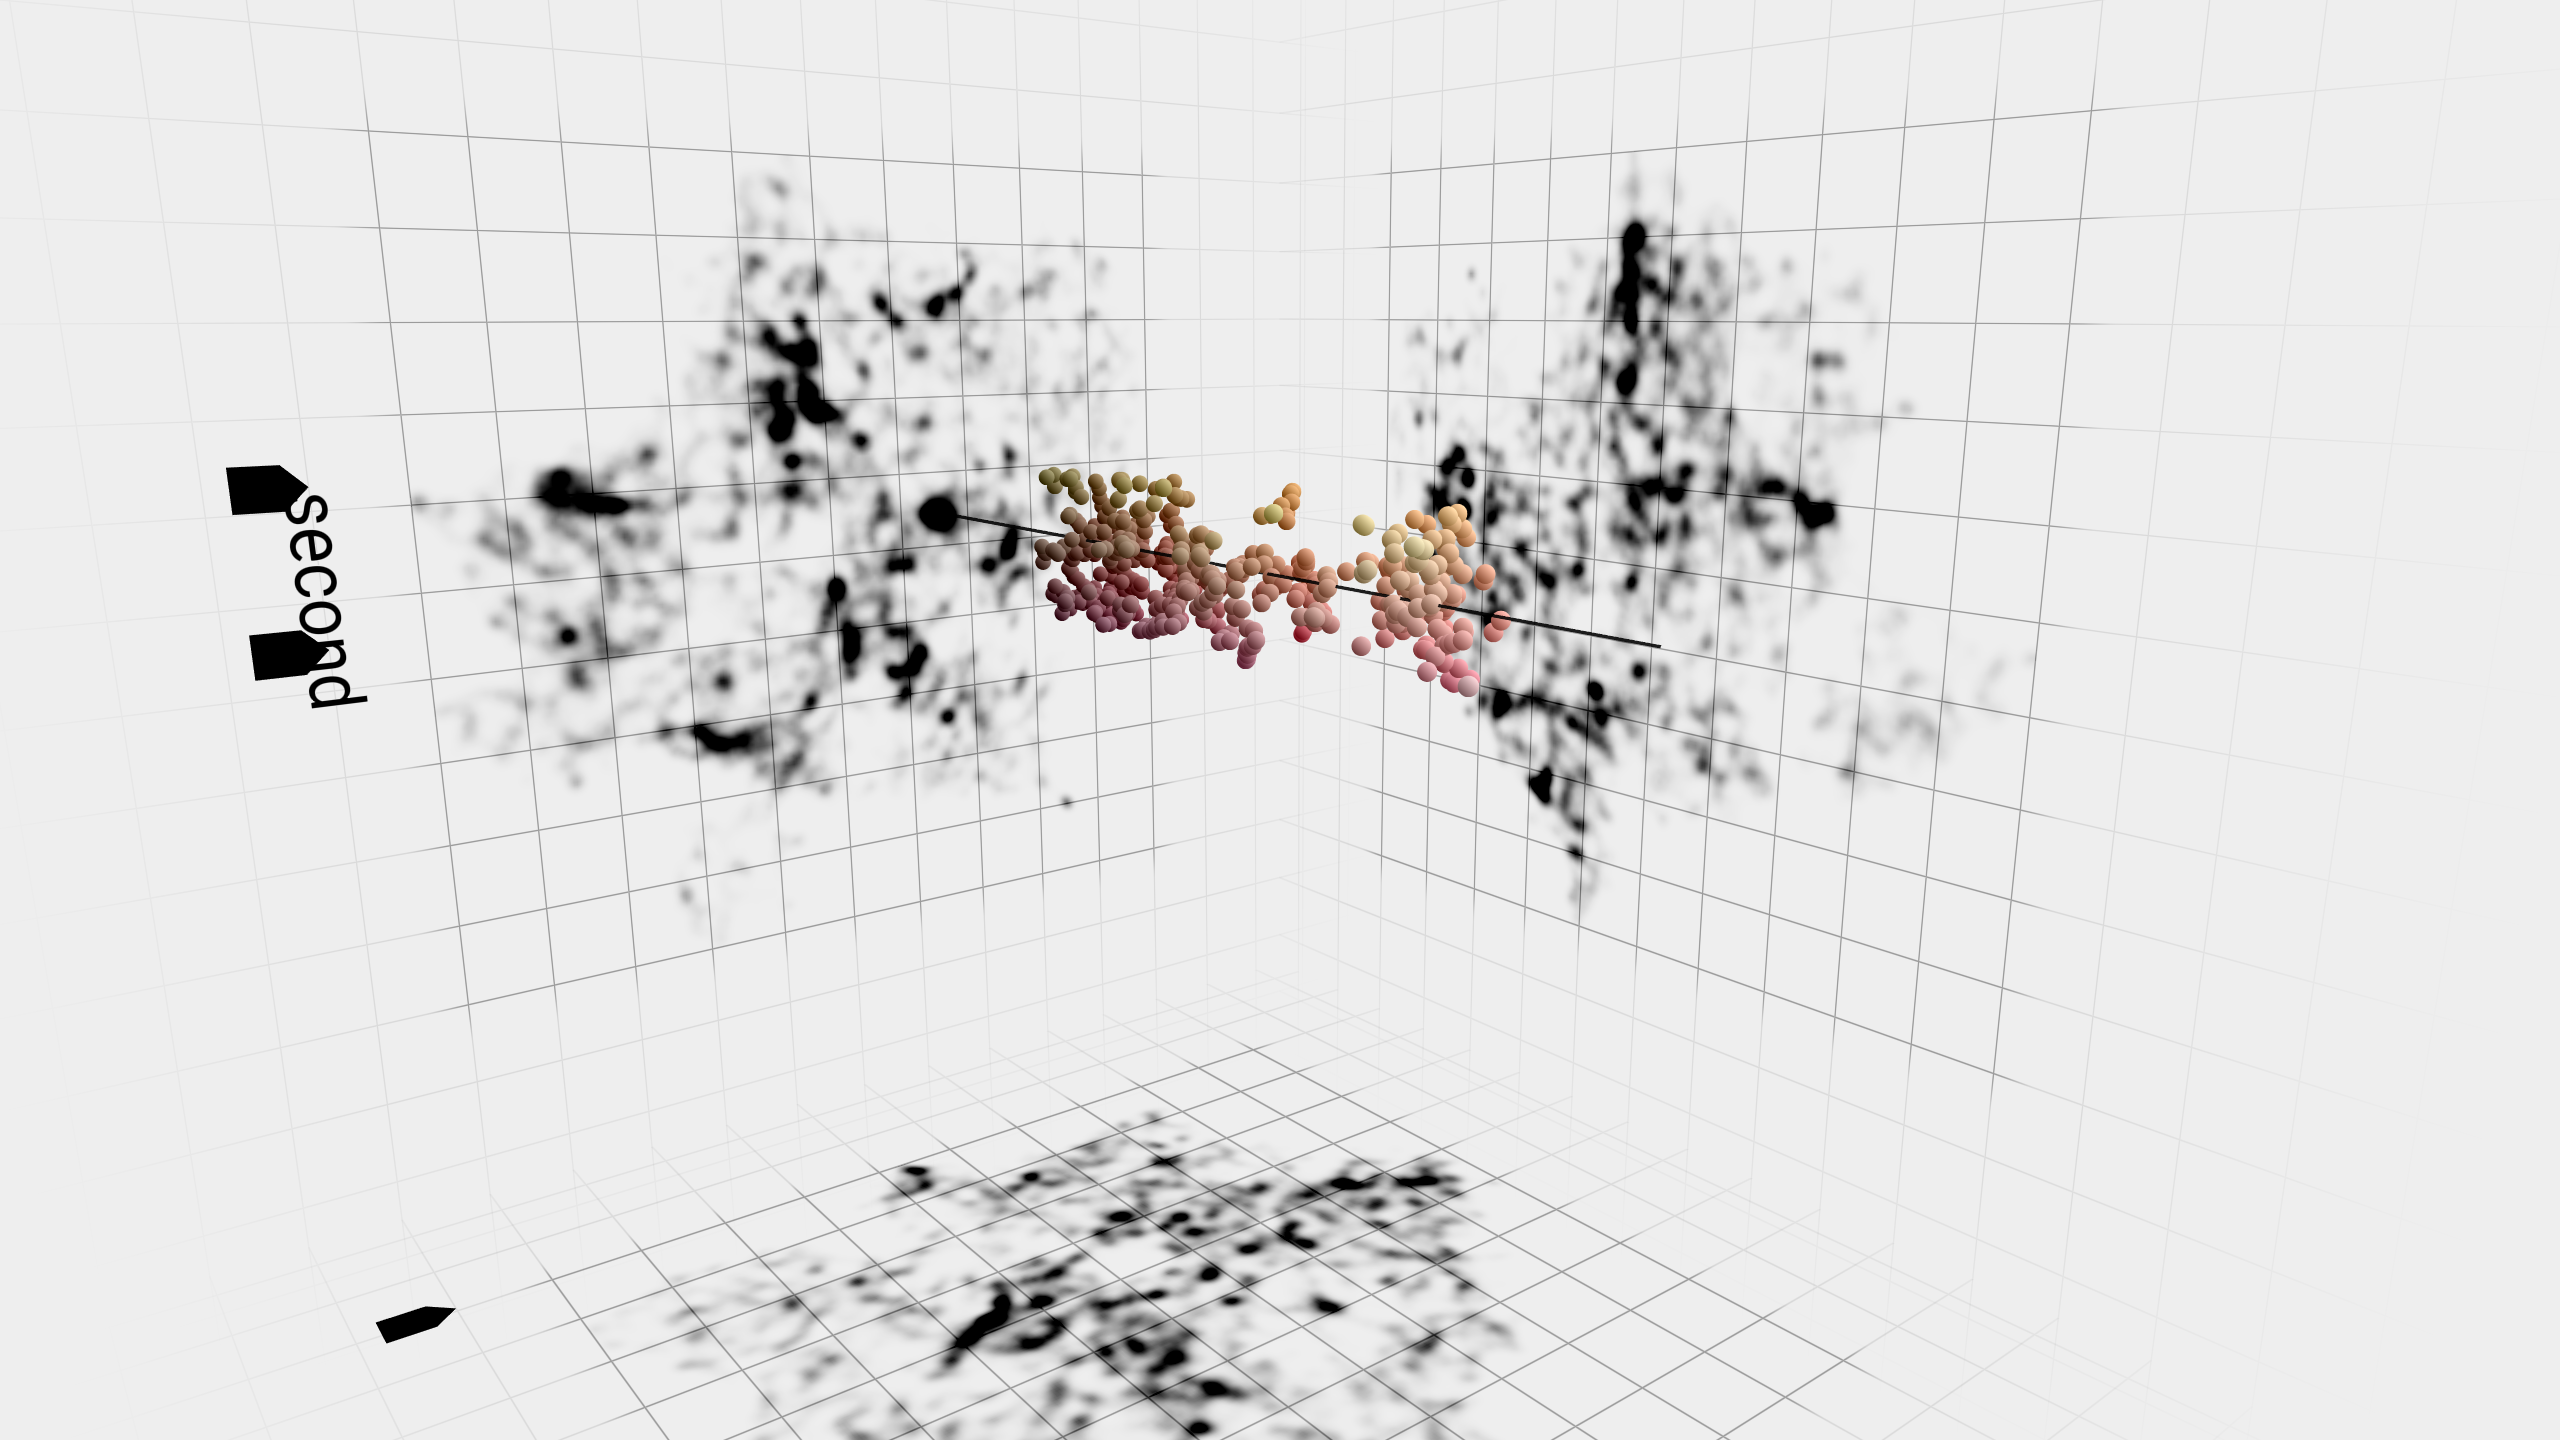
\includegraphics[width=\linewidth,trim={25cm 25cm 20cm 15cm},clip]{figures/refline_grid.png}
  \caption{By placing a reference line onto any of the density maps, the points composing a cluster can be deducted.}
  \label{fig:reflineGrid}
\end{figure}

\section{Implementation}
\label{sec:impl}

Our implementation uses WebGL~2 to provide a web-based data set introspection tool \cite{scatterplot}.
Depending on the GPU, screen resolution and rendering settings, the maximum number of data points for interactive rendering ranges from 1 million to above 50 million.

\paragraph{Density Maps.}
The density maps are generated by additional render passes, using axis aligned orthographic projections.
Thus, each vertex has to be rendered four times instead of once.
However, as the density maps do not change once the data set is loaded, the additional render passes can be run once instead of on every frame.
For encoding the density maps, we chose a 16-bit floating point RGB texture, with each channel storing one of the three maps (\autoref{fig:orthoDebug}).
In order to count the data points overlapping at any position in the resulting density map, we utilize additive blending, which requires configuring the blending function to {\small\texttt{gl.blendFunc(gl.ONE, gl.ONE)}}.
This results in all density values being added up without being influenced by alpha blending.

\paragraph{Density Gradients.}
To create density gradients, we encode the distance to the point's center instead of drawing each data point as a uniform area---similar to how metaballs are created.
Instead of an inverse falloff, however, we chose a linear falloff.
This results in a smoother density map, having close points melt together earlier.
An inverse falloff function would result in more abrupt density changes, with points staying separated longer but merging quicker once their distance falls under a threshold.

\begin{figure*}
  \centering
  \begin{subfigure}[t]{0.243\linewidth}
    \centering
    \tikzsetnextfilename{density-r}
    \begin{tikzpicture}[inner sep=0pt, outer sep=0pt,
        spy using outlines = {magnification = 4.0, size = 1.75cm, connect spies,every spy on node/.append style={thick}}
    ]
        \node[] (front) { 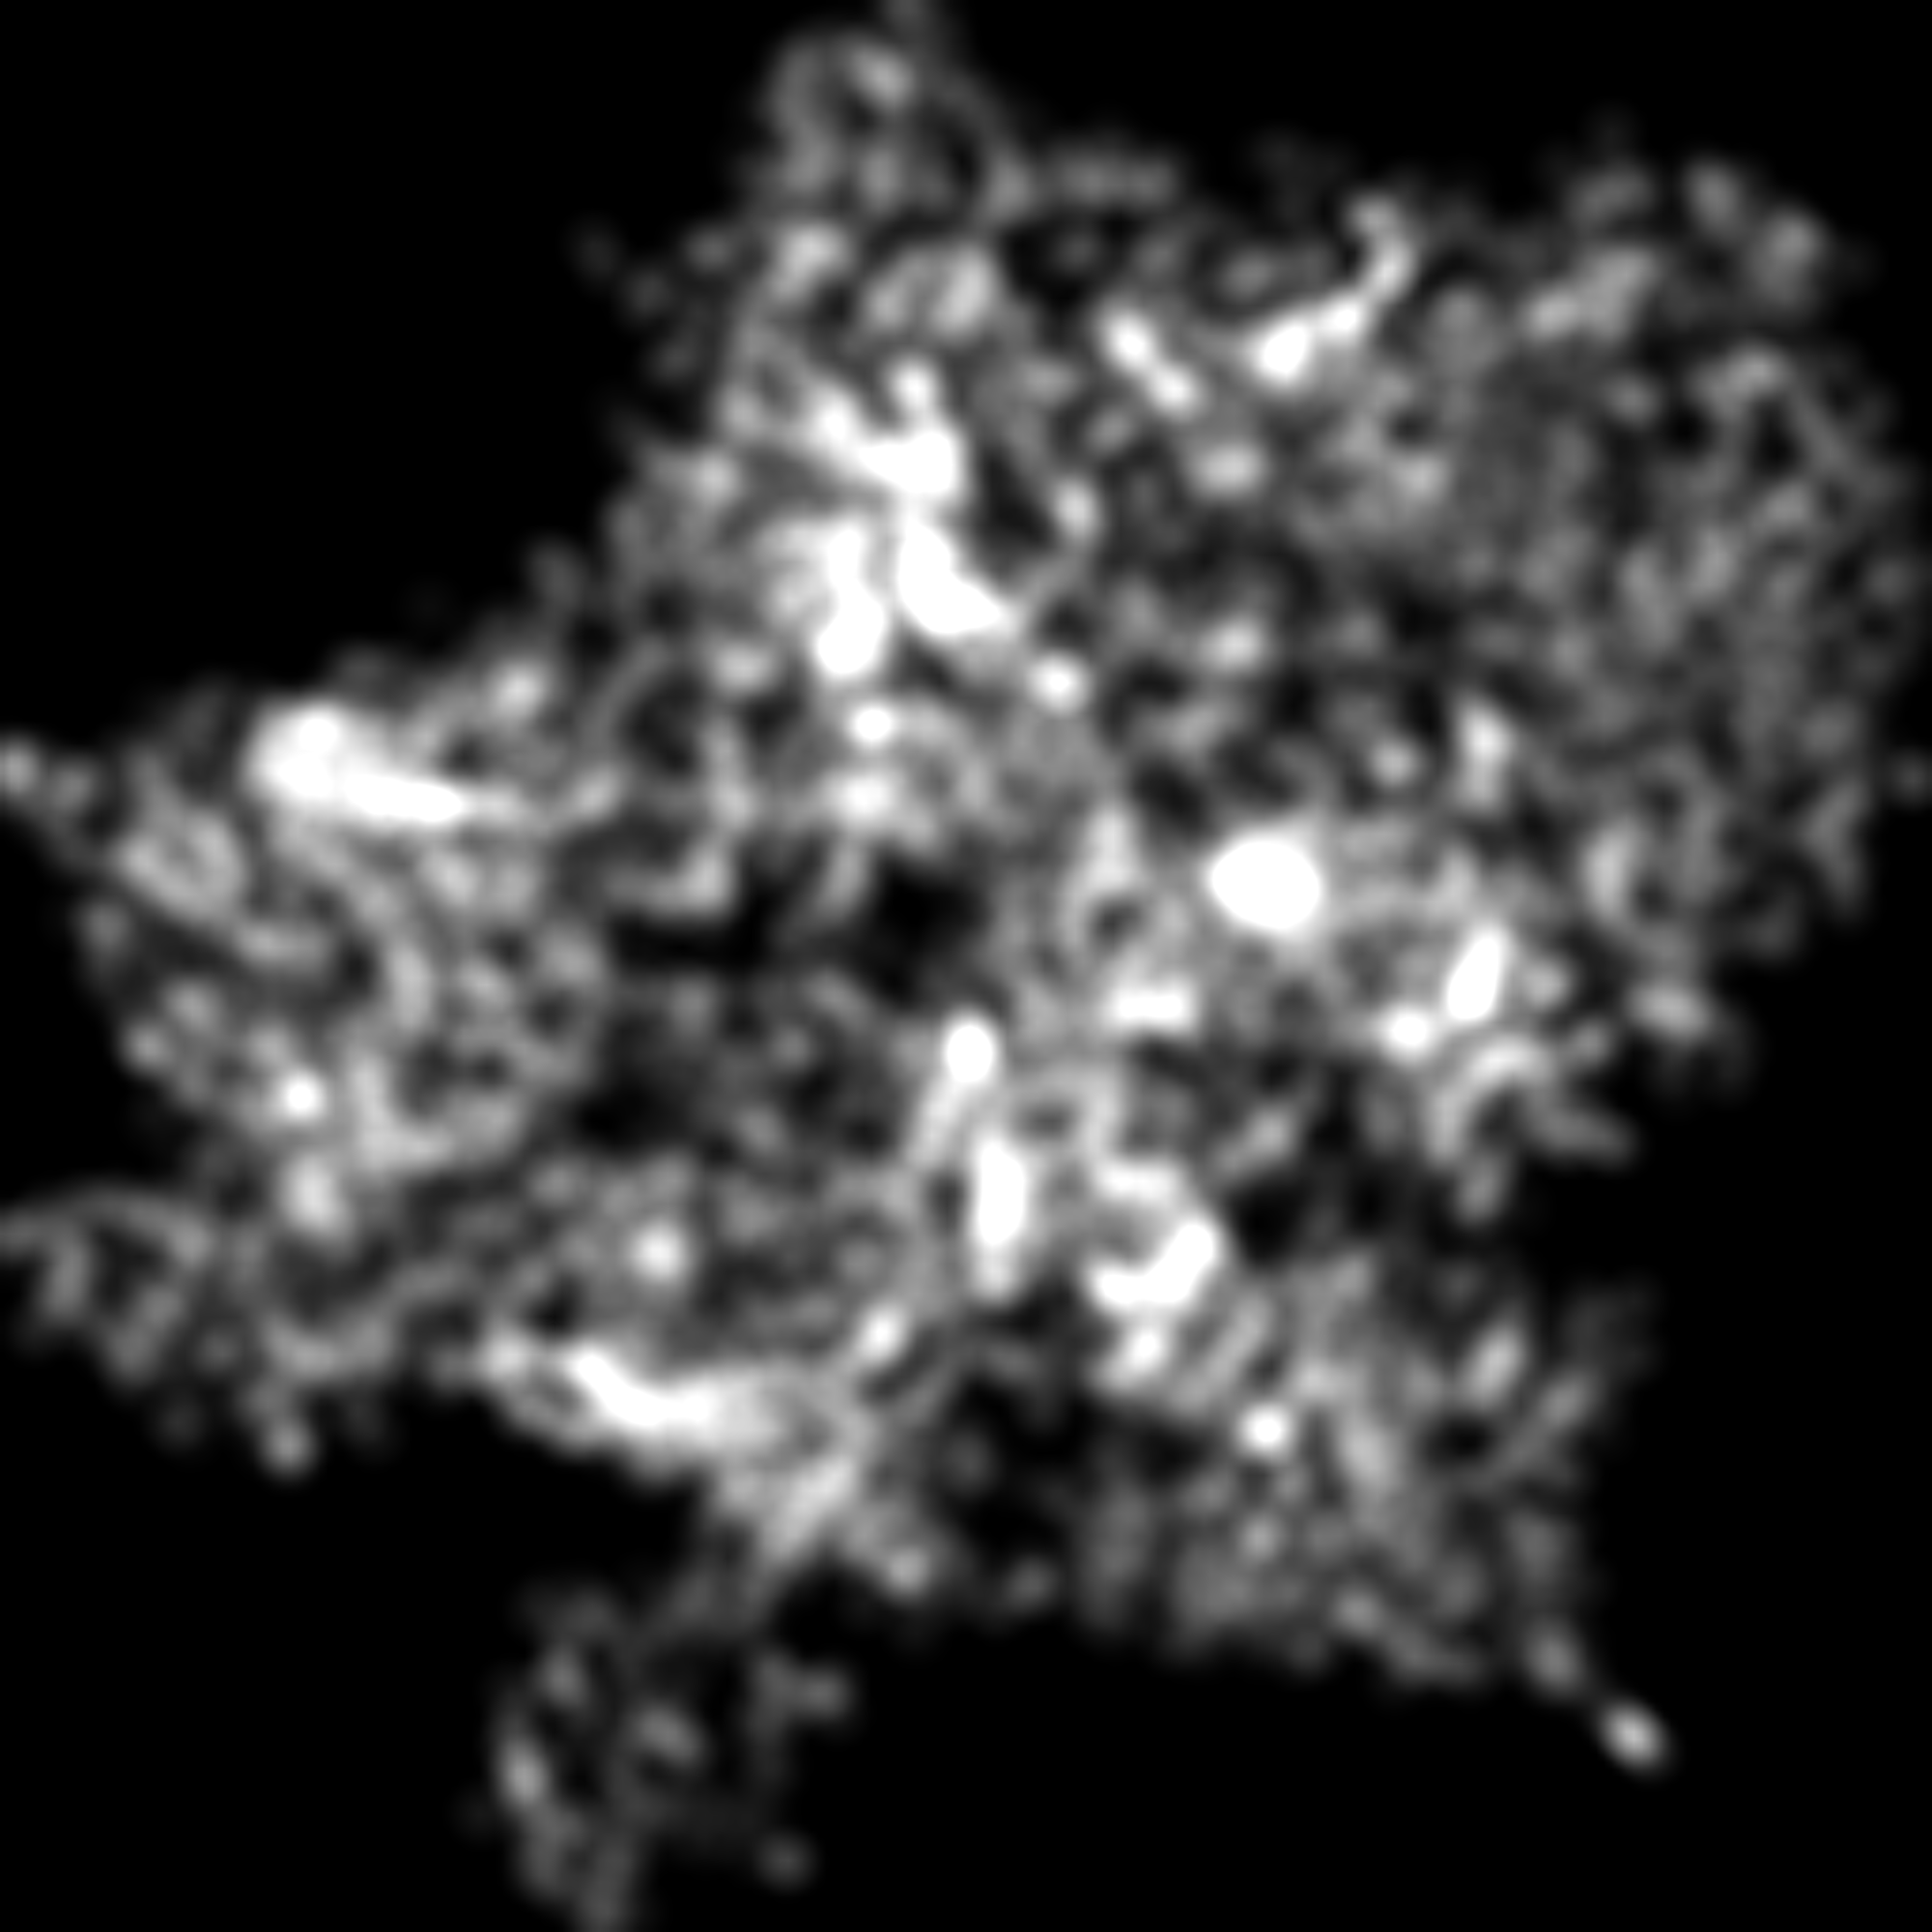
\includegraphics[width=0.6\linewidth]{figures/ortho_5percent_r.png} };
        \spy[red] on ($(front.center)+(0.0mm, 0.0mm)$) in node at ($(front.center)+(+2.0cm,-0.82cm)$);
        \node[] at ($(front.center)+(2.1cm,0.6cm)$) { \huge $\bigoplus$ };
    \end{tikzpicture}
    \caption{Red channel contains front view (x points right, y points up)}
  \end{subfigure}
  \hfill
  \begin{subfigure}[t]{0.243\linewidth}
    \centering
    \tikzsetnextfilename{density-g}
    \begin{tikzpicture}[inner sep=0pt, outer sep=0pt,
        spy using outlines = {magnification = 4.0, size = 1.75cm, connect spies,every spy on node/.append style={thick}}
    ]
        \node[] (side) { 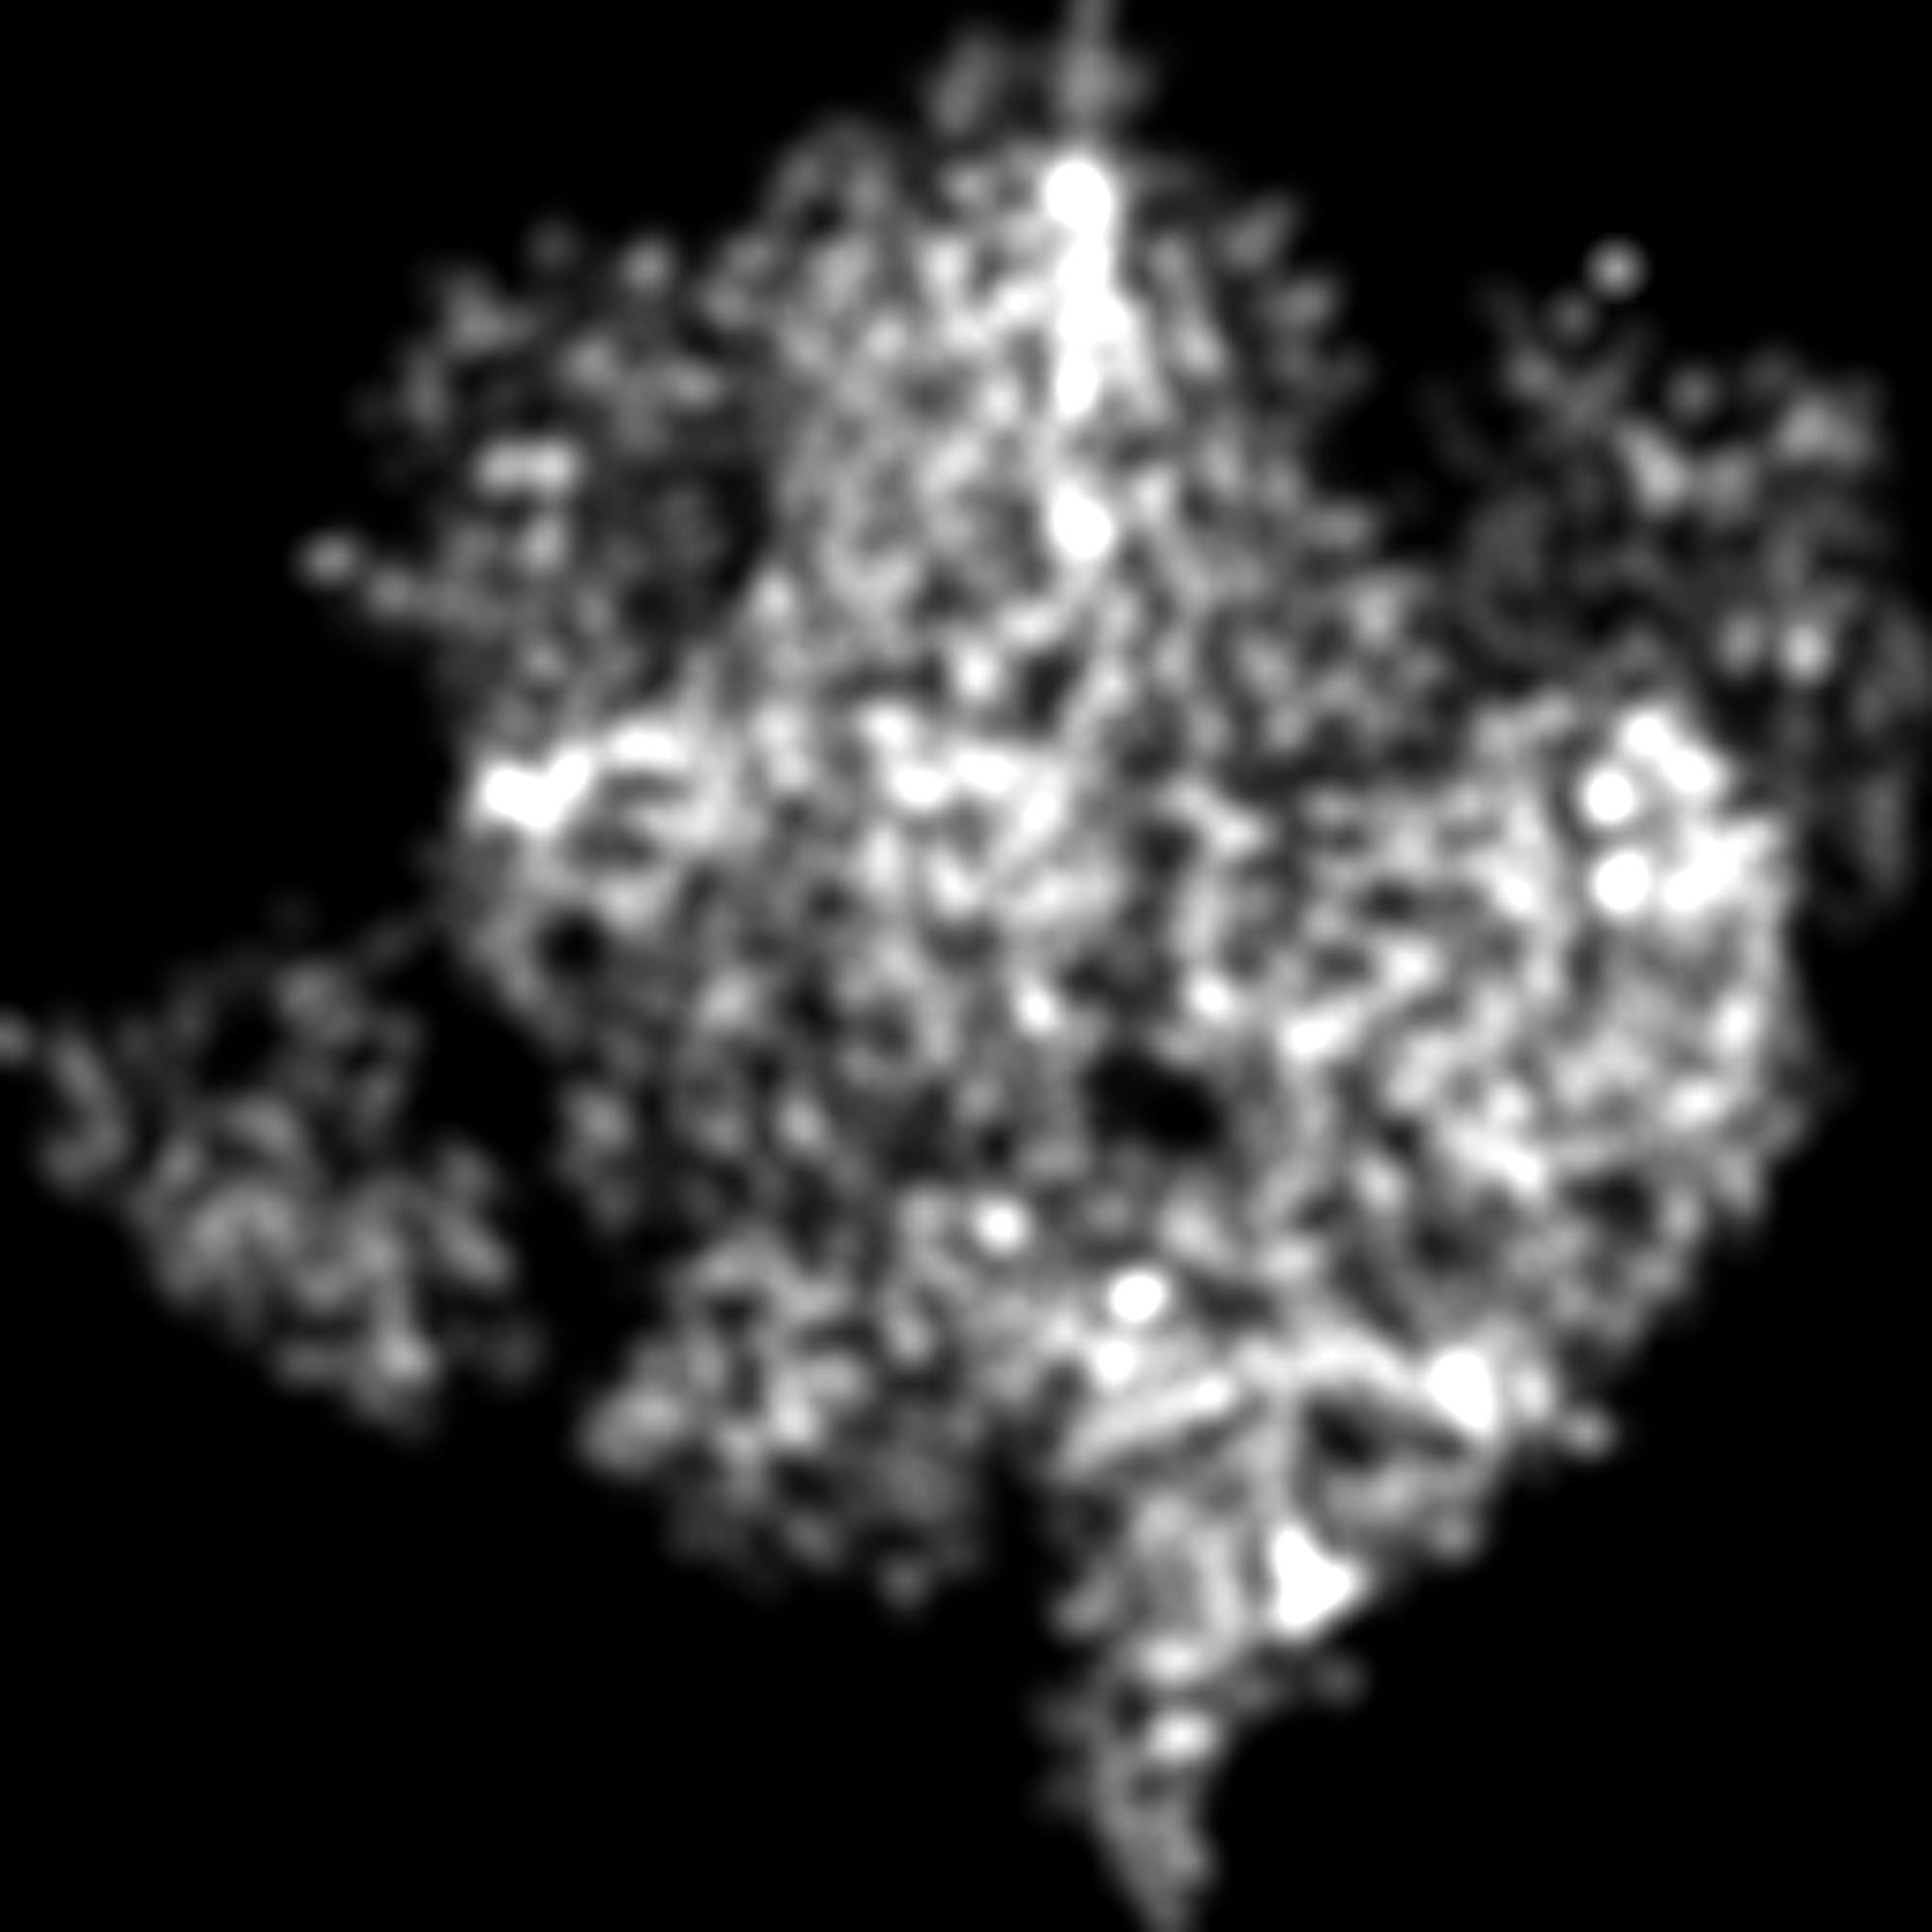
\includegraphics[width=0.6\linewidth]{figures/ortho_5percent_g.png} };
        \spy[green] on ($(side.center)+(0.0mm, 0.0mm)$) in node at ($(side.center)+(+2.0cm,-0.82cm)$);
        \node[] at ($(side.center)+(2.1cm,0.6cm)$) { \huge $\bigoplus$ };
    \end{tikzpicture}
    \caption{Green channel contains side view (z points left, y points up)}
  \end{subfigure}
  \hfill
  \begin{subfigure}[t]{0.243\linewidth}
    \centering
    \tikzsetnextfilename{density-b}
    \begin{tikzpicture}[inner sep=0pt, outer sep=0pt,
        spy using outlines = {magnification = 4.0, size = 1.75cm, connect spies,every spy on node/.append style={thick}}
    ]
        \node[] (top) { 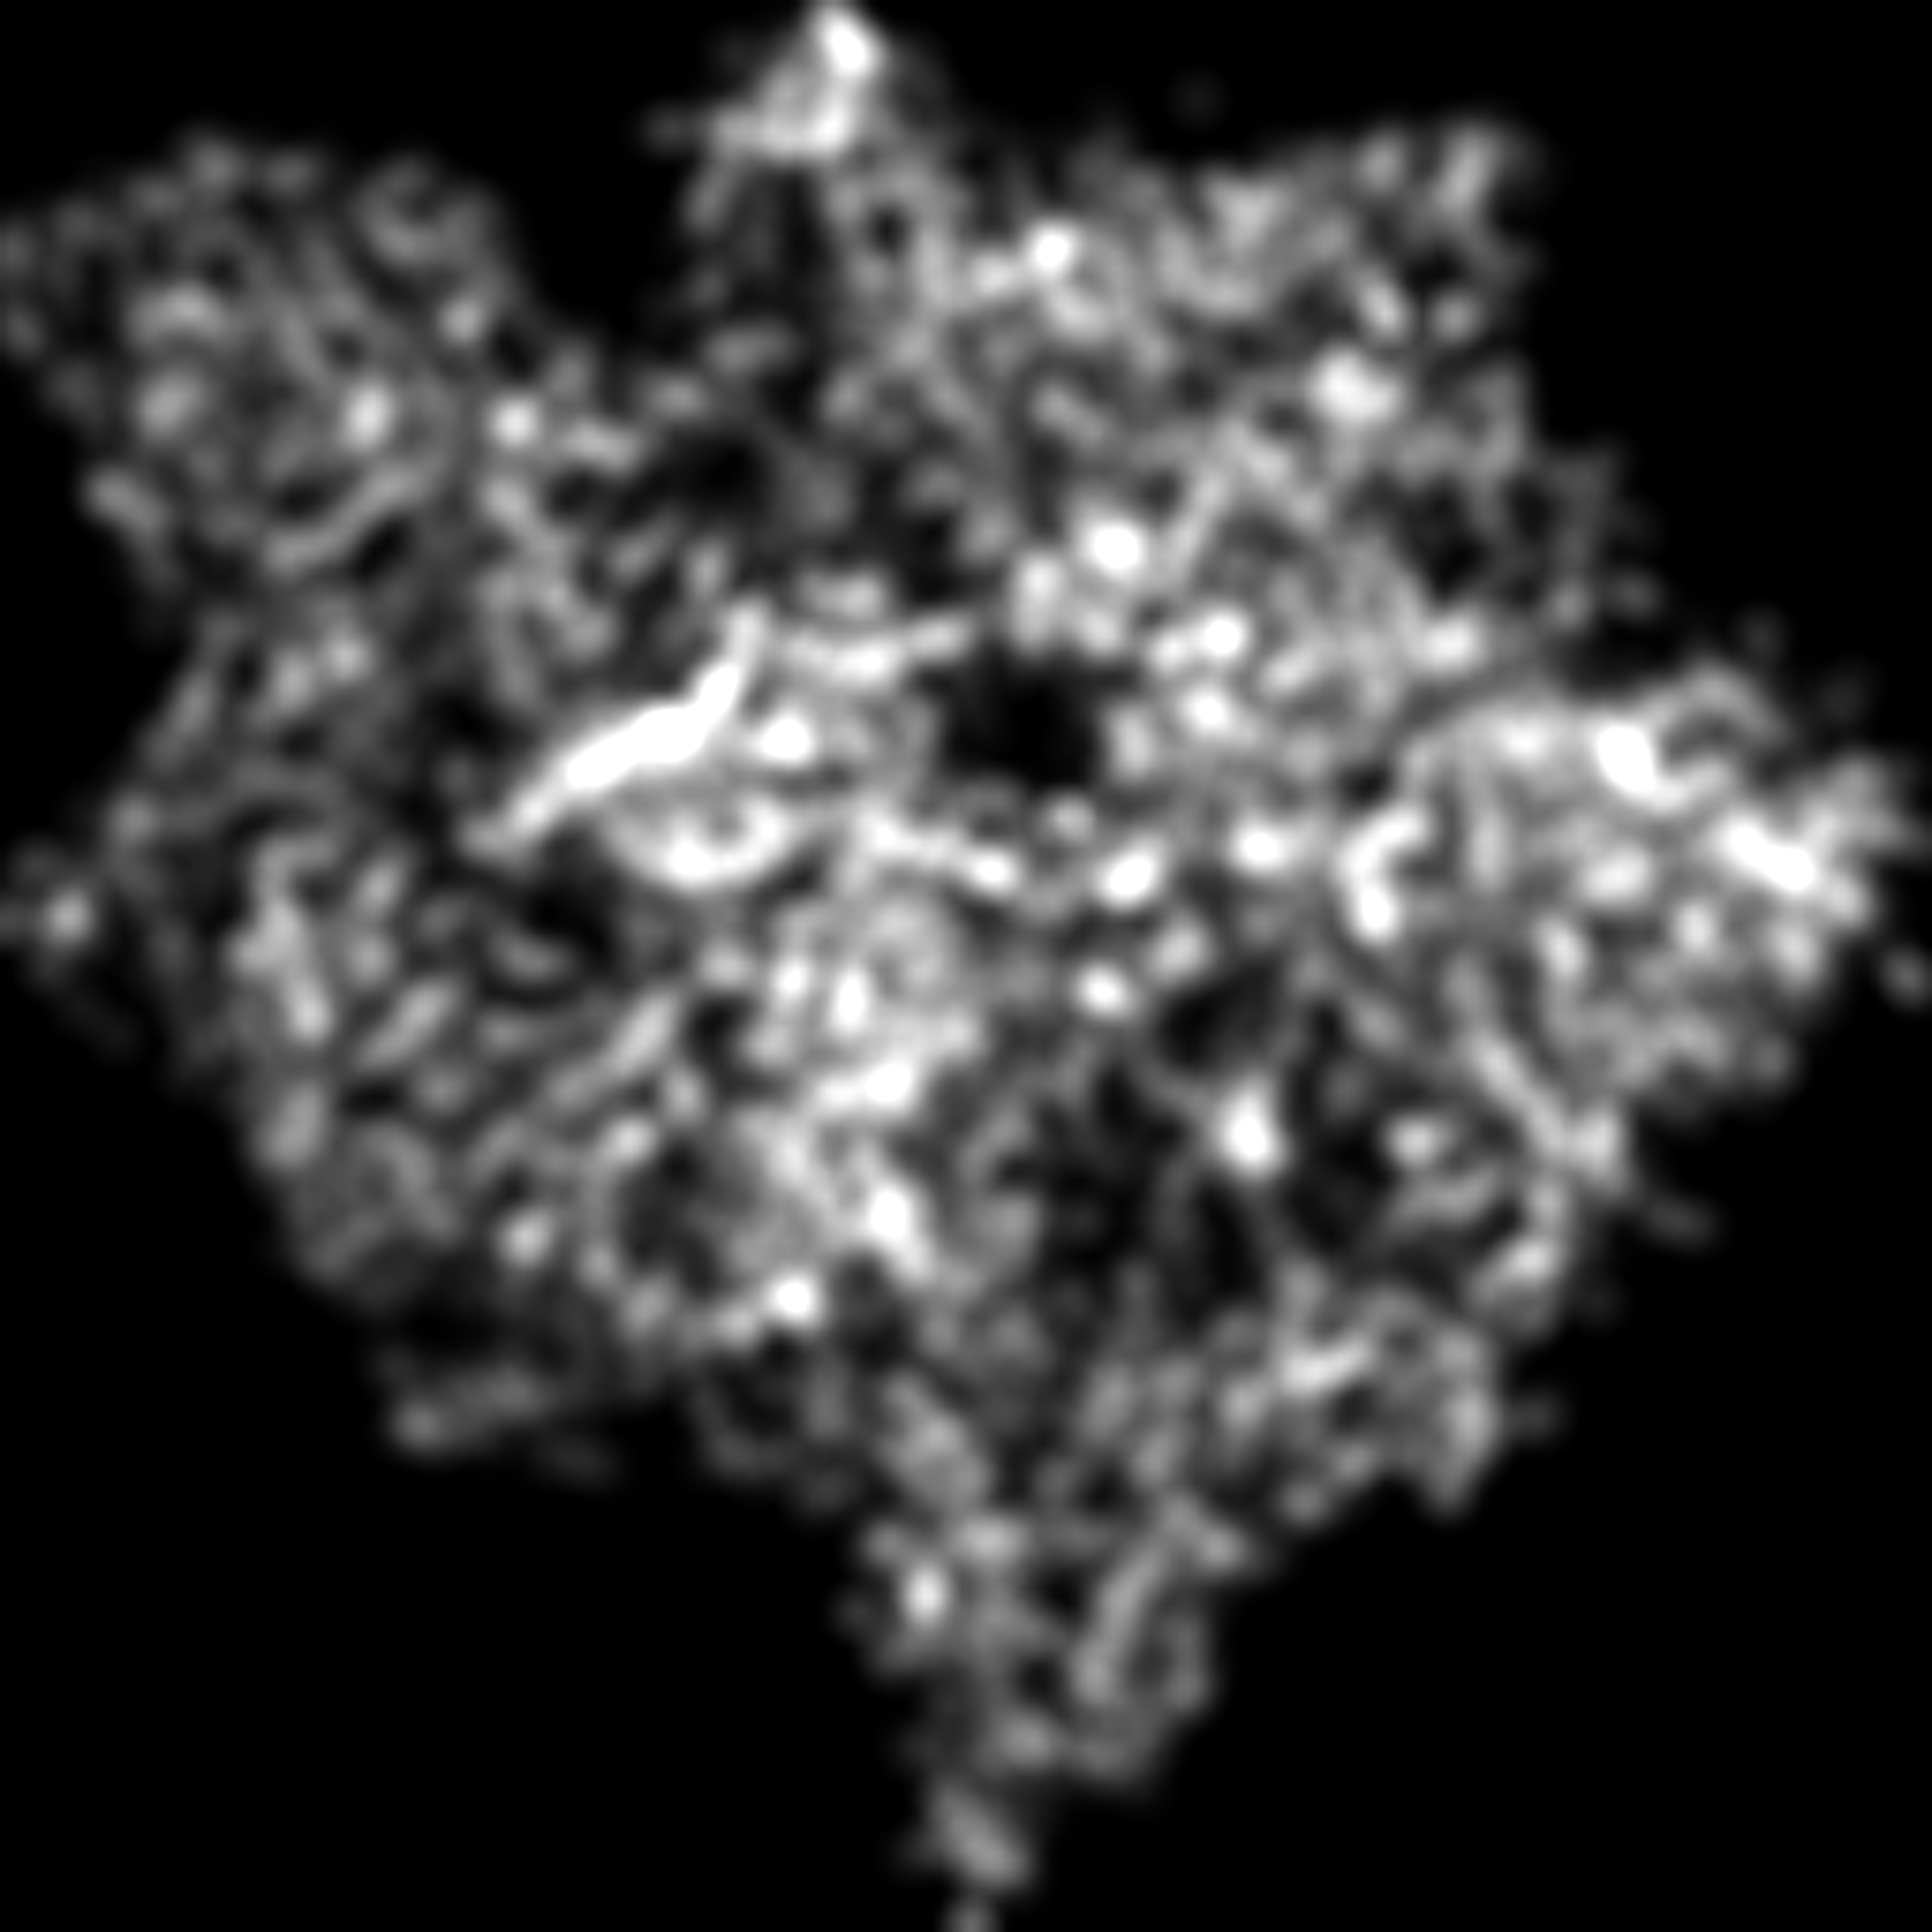
\includegraphics[width=0.6\linewidth]{figures/ortho_5percent_b.png} };
        \spy[blue] on ($(top.center)+(0.0mm, 0.0mm)$) in node at ($(top.center)+(+2.0cm,-0.82cm)$);
        \node[] at ($(top)+(2.1cm,0.6cm)$) { \huge $\Rightarrow$ };
    \end{tikzpicture}
    \caption{Blue channel contains top view (x points right, z points down)}
  \end{subfigure}
  \hfill
  \begin{subfigure}[t]{0.243\linewidth}
    \centering
    \tikzsetnextfilename{density-combined}
    \begin{tikzpicture}[inner sep=0pt, outer sep=0pt,
        spy using outlines = {magnification = 4.0, size = 1.75cm, connect spies,every spy on node/.append style={thick}}
    ]
        \node[] (full) { 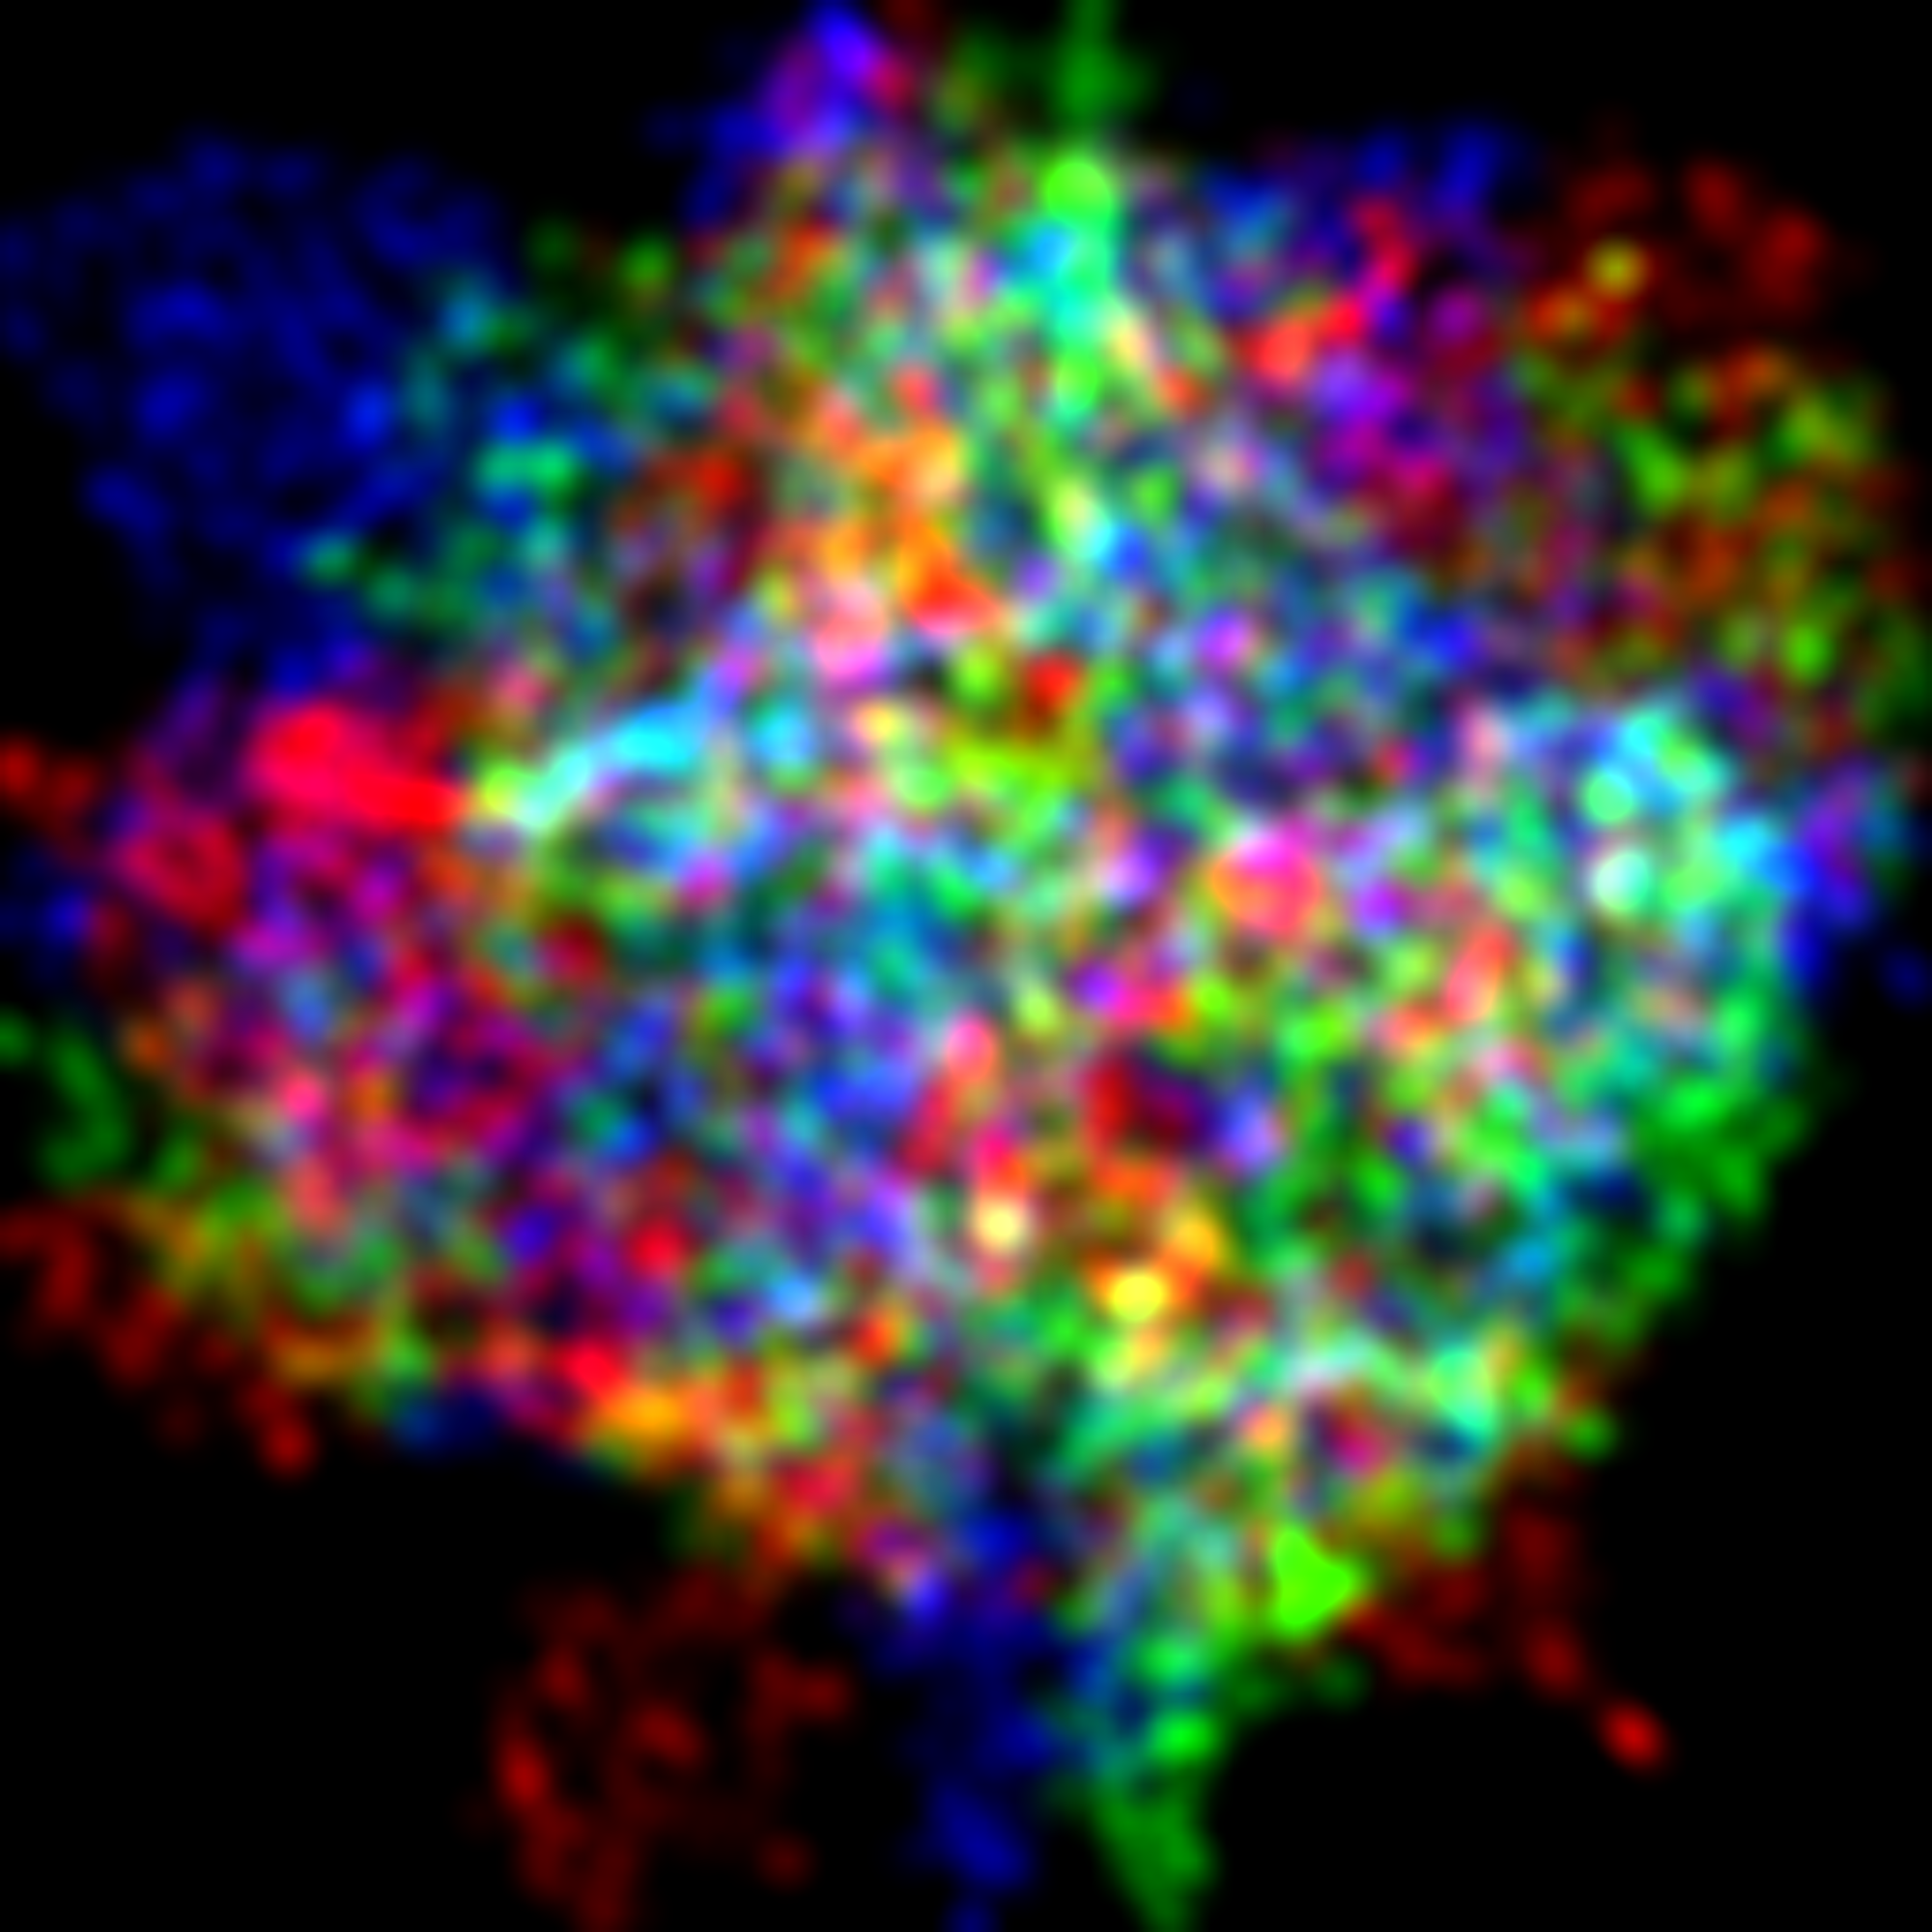
\includegraphics[width=0.7\linewidth]{figures/ortho_5percent.png} };
        \spy[white] on ($(full.center)+(0.0mm, 0.0mm)$) in node at ($(full.center)+(+1.8cm,-0.66cm)$);
    \end{tikzpicture}
    \caption{Combined texture containing all three density maps.}
  \end{subfigure}
  \vspace{-0.5\baselineskip}
  \caption{Packed density maps, each color channel storing one map. The values are scaled down to 5~\%, however, some areas still appear blown out, as the number of data points at that position exceeds the [0,~1] range typically expected in an RGB texture.}
  \label{fig:orthoDebug}
\end{figure*}

\paragraph{Density Maps Scaling.}

In order to provide a useful default scaling for the density maps, the density should be normalized.
This requires the maximum density to be determined.
A trivial approach would be to read back all texels from the GPU's memory and calculate the maximum using the CPU.
Instead, we render the texture to a lower resolution texture using a screen aligned quad, with each output texel calculated as the maximum of an $n\times{}n$ kernel, $n$ being the ratio between the textures' resolutions.
For example,
a $512\times512$ texture
can be reduced to a single value using three passes with an $8\times8$ kernel ($512 \rightarrow 64 \rightarrow 8 \rightarrow 1$). 
The value can then be read back. 
This is a common approach to GPU-accelerated reduction \cite{scatterjs,gpuGems}.
Dividing by the maximum density gives a sensible default scaling for the density values, each ranging between 0 and 1.
The scaling can also be adjusted using strength and gamma adjustments, as known from image manipulation.

\paragraph{Color Schemes.}

The different color schemes can be realized by providing an $n \times 1$-texture to the fragment shader.
This texture is filled with values on the CPU side.
Resizing the texture and disabling linear filtering allows for lower color resolution (\autoref{fig:colorSpectral7}).

\paragraph{Interaction.}

Point selection is implemented using an ID buffer.
IDs are stored as 32-bit unsigned integers, resulting in an maximum supported point count of over 4 billion.
If more distinct IDs are required, the IDs could be split into a high and low part, which are stored as separate variables.
By reading back the pixel below the mouse cursor, the currently active data point can be determined.
For placing reference lines on the density maps, this approach is reused.
Reading this data back from the GPU allows discerning where the user clicked, as well as on which of the three planes.
As the IDs are stored as an 32-bit integer, this data is packed into the same amount of bits.
One byte is used to store the grid ID.
The remaining 3 bytes store the x and y position on the grid, each encoded as a 12-bit integer.
The precision of 4096 different positions per axis is enough for typical rendering scenarios.

\paragraph{Reference Lines.}
For rendering the reference lines, the points' vertex attribute array is rebound with an offset based on the selected ID.
This allows reusing the data already present in GPU memory.
Setting a coordinate's value to the respective grid's position results in a perpendicular line, which is repeated for all three grids.

\section{Evaluation}
\label{sec:eval}

This evaluation is split into two parts. First, we assess whether 16-bit floating point textures provide enough precision for our use case. Afterwards, we discuss this technique's performance impact.

\paragraph{Density Map Precision.}

When describing the density map generation, we noted that it is stored as an 16-bit floating point texture.
In comparison with a 32-bit integer texture, this means a significant drop in precision.
Even when using a 32-bit floating point texture, only 24 bits are used to store the mantissa (counting the hidden bit)\footnote{\href{https://www.khronos.org/opengl/wiki/Small_Float_Formats}{www.khronos.org/opengl/wiki/Small\_Float\_Formats}}.
This affects how many points can overlap before any data loss occurs.
The required precision is dependent on both the point size and the falloff function, as well as the target number of decimal places.
Storing 32-bit fixed point numbers with a precision of 0.01 would allow over 40 million points to overlap, while allowing each point to contribute a full density of 1 ($n = 2^{32}*0.01$).
However, WebGL~2 does not support blending of any type for integer textures.
This means we can't utilize additive blending to aggregate density values in an integer texture and therefore must build on floating point textures.
A 32-bit floating point number however only allows for around 168 thousand overlapping points before data loss occurs at the second decimal ($n = 2^{24}*0.01$).

32-bit textures introduce an additional issue, as WebGL~2 does not support bi-linear interpolation\footnote{\href{https://www.khronos.org/registry/OpenGL-Refpages/es3.0/html/glTexImage2D.xhtml}{www.khronos.org/registry/OpenGL-Refpages/es3.0/html/glTexImage2D.xhtml}}.
This results in pixelated density maps.
It is possible to manually implement the linear filtering inside the fragment shader, however this results in a performance impact.
In order to utilize hardware-accelerated interpolation, the bit-depth must be reduced to 16.
This, in turn, reduces the mantissa to 11 bits (again including the hidden bit), resulting in a significantly lower number of overlapping points of 20 ($n = 2^{11}*0.01$).
While heavily reduced, this precision could still be considered acceptable based on the number of data points and point size.
Assuming a normal distribution,
around 0.04~\% of points affect the center pixel\footnote{
  Resolution 512~px, 5~px point size.
  Using a mean of 255,5 and a standard derivation of 100, approximately 2~\% of points fall into the [253, 258] range, affecting the center pixel.
  Extending this to 2D results in only $0.02*0.02$, or 0.04~\% of points.
  See \href{https://onlinestatbook.com/2/calculators/normal_dist.html}{onlinestatbook.com/2/calculators/normal\_dist.html}
}.
A resolution of 11 bit thus is sufficient for data sets of up to 50 thousand points ($n = 2^{11}*0.01/(0.02^2)$).
Relaxing the precision requirement to 1 digit increases this to 500 thousand points.

To support more points, the density calculation could
use multiple frame buffers and distribute the points heuristically, e.g., based on the point ID.
These could be added up in a post processing step.

In order to implement the distribution of points as minimally invasive as possible, one possible approach would be to extend the frame buffer by additional attachments. Based on the the chosen heuristic, the fragment shader writes only to one of them. This requires no adjustments to the underlying rendering process. This approach, however, is restricted by the maximum possible number of color attachments. The OpenGL ES 3 specification (which WebGL~2 is based on) requires \texttt{MAX\_COLOR\_ATTACHMENTS} to be at least 4, with modern devices often supporting more attachments.%

\paragraph{Performance.}
The density map calculation takes less time than rendering the 3D scene.
This results from a reduced resolution (e.g., $256\times256$ instead of $1920\times1080$, resulting in a fragment reduction by factor $31.6$), as well as the simpler fragment shader. 
On top of this, the density maps can be cached and reused as long as the underlying data is unchanged.
In practice, this means that the density maps' performance impact is limited to texture lookups when drawing the grids.
Thus, we confirmed earlier performance measurements, meaning that millions of data points can be interactively visualized on mid-range consumer hardware \cite{scatterplot}.

\section{Conclusions}
\label{sec:conclusion}

This paper proposes a novel technique for exploring 3D scatter plots suffering from occlusion.
We extended the existing approach of mapping 2D scatter plots onto axis-aligned grids with enhancements for resolving 2D over-plotting issues.
This results in density maps, condensing individual points into an overview of the data set's structure.
We combined this with interaction techniques for filtering and referencing data points based on the density maps.
This approach facilitates the discovery and exploration of data sets.

The proposed techniques provide the user with an overview of the data set.
This approach works alongside the 3D scatter plot but does not actively affect it.
A more active interaction could further improve data set comprehension, e.g., by affecting visual components based on density.
One possible enhancement is reducing the opacity of data points in low-density areas, resulting in a scatter plot focused on high-density clusters.
Instead of displaying the density maps, the bounding planes could also be used to display additional data, such as aggregated point data.
A comparison of different density falloff functions could also be worthwhile.
The current implementation uses a linear falloff based on the intent of counting overlapping data points.
Another option, inspired by metaballs, is the inverse squared euclidean distance.

\begin{acks}
This work was funded by the German Federal Ministry of Education and Research (BMBF, KMUi) within the project \enquote{Knowhow-Analyzer}.
This work is part of the \enquote{Software-DNA} project, which was funded by the European Regional Development Fund (ERDF -- or EFRE in German) and the State of Brandenburg (ILB).
This Project is supported by the Federal Ministry for Economic Affairs and Climate Action (BMWK, ZIM) on the basis of a decision by the German Bundestag.
\end{acks}

\bibliographystyle{ACM-Reference-Format}
\bibliography{references}

\appendix
\end{document}
\endinput
